%% \chapter[htoc-titlei][hhead-titlei]{htitlei}
%% -----------------------------------------------------------------------------
\chapter[Measurement of same-sign $WW$ production at $\sqrt{s} = 13~\mathrm{TeV}$ with ATLAS][Measurement of same-sign $WW$ production at $\sqrt{s} = 13~\mathrm{TeV}$ with ATLAS]{Measurement of same-sign $WW$ production at $\sqrt{s} = 13~\mathrm{TeV}$ with ATLAS}
\label{ch:ssww13tev}

Production of same-sign $W$ boson pairs is a particularly interesting SM process, especially when produced via vector boson scattering (VBS).
The VBS \ssww process is particularly sensitive to the electroweak symmetry breaking (EWSB) mechanism as well as potential ``beyond the Standard Model'' (BSM) physics.
The first evidence of electroweak (EWK) \ssww production was seen by the ATLAS and CMS experiments at \com{8} with exesses of $3.6\sigma$~\cite{2014.ssww-8tev-atlas} and $2.0\sigma$~\cite{2015-ssww-8tev-cms} over backgrounds, respectively.
More recently, ATLAS and CMS have both observed the EWK process at \com{13} with significances of $6.9\sigma$~\cite{2018.ssww-13tev-atlas-conf} and $5.5\sigma$~\cite{2017.ssww-13tev-cms}, respectively.
The analysis presented in this chapter is based off of the ATLAS \com{13} observation and cross section measurement of EWK \ssww production~\cite{2018.ssww-13tev-atlas-conf, 2018.ssww-13tev-atlas-support}.

\section{Analysis Overview}\label{ssww13tev:overview}
\subsection{Experimental overview of vector boson scattering}\label{ssww13tev:vbs_theory}
VBS processes are very important to understand due to their sensitivity to the EWSB mechanism.
As explained in Section~\ref{sec:theory_vbs}, in the absence of a light SM Higgs boson, the scattering amplitude of longitudinally polarized vector bosons grows with center-of-mass energy. % and ultimately violates unitarity above \com{1} in the absence of a light SM Higgs boson.
However, once the Higgs is introduced, the divergences cancel and the cross section no longer grows unbounded. %~\cite{1977.ben-lee-weak-interactions, 2009.strong-gauge-boson-scattering}. % i already cited these guys earlier when saying the same thing

With the discovery of the Higgs boson in 2012~\cite{HIGG-2012-27, CMS-HIG-12-028}, the EWSB mechanism can now be directly studied.
Due to the potential exchange of a Higgs boson in the VBS diagrams (\ssww itself does not contain the $s$-channel diagram), VBS processes are directly sensitive to properties of the Higgs.
For example, the high-mass tail in the $VV$ scattering system allows an approximation of the effective coupling strength of the Higgs to vector bosons that is independent of any assumptions on the Higgs width~\cite{2015.higgs-constraints-from-vbs}.
Additionally, the center of mass energy dependence of the $VV$ scattering can reveal whether the Higgs boson unitarizes the longitudinal scattering amplitude fully or only partially~\cite{2014.higgs-WW-scattering-theory}.

VBS events are characterized by two quarks from the colliding protons each radiating a vector boson which then scatter and decay in the detector.
The incoming quarks carry a large amount of momentum and only deflect a small amount upon emitting the vector boson; as a result, they often enter the calorimeters very close to the beam line.
Ignoring the decay products of the scattered bosons for now, these VBS events result in a final state of two vector bosons ($V$) and two jets ($j$) at high pseudorapidities (called \emph{forward jets} or \emph{tag jets}) from the outgoing quarks.
The shorthand $VVjj$ is used to represent this final state.
%A visual representation of a typical event topology for a \ssww event can be seen in Figure~\ref{fig:ssww13tev_event_topology}.

$VVjj$ events can be produced via two different physical processes.
The first involves purely electroweak interactions in the tree-level diagrams, with $\mathcal{O}(\alpha_{\textrm{EWK}}) = 6$ %(including the decays of the bosons).
and will be referred to as \emph{EWK production}.
This can be further broken down into VBS and non-VBS production.
In the VBS EWK production, the scattering occurs via triple or quartic gauge couplings, as well as the $s$- or $t$-channel exchange of a Higgs boson.
%These diagrams are shown in Figure~\ref{fig:ssww13tev_diagrams_vbs}.
The non-VBS EWK production contains the same final state of two vector bosons and two outgoing quarks, but the bosons do not scatter.
Due to gauge invariance, it is not possible to separate the VBS from the non-VBS productions~\cite{2006.isolating-vbs-lhc}; therefore, both are included in the signal generation and are indistinguishable from one another.
The second process involves a mix of the EWK and strong interactions, of order $\mathcal{O}(\alpha_s) = 2 \otimes \mathcal{O}(\alpha_{\textrm{EWK}}) = 4$ and will be referred to as \emph{QCD production}.
The tree-level Feynman diagrams for VBS EWK, non-VBS EWK, and QCD $VVjj$ production are found in Figures~\ref{fig:ssww13tev_diagrams_vbs}, \ref{fig:ssww13tev_diagrams_ewk}, and \ref{fig:ssww13tev_diagrams_qcd}, respectively.

\begin{figure}[htbp]
  \centering
  \includegraphics[width=.8\textwidth]{figs/ssww_13tev/diagrams/Vbscore}
  \caption{Tree-level Feynman diagrams for VBS EWK $VVjj$ production including triple gauge couplings involving $W$ and/or $Z$ bosons (top left and top middle), quartic gauge coupling (top right), or the exchange of a Higgs boson ($s$-channel bottom left and $t$-channel bottom right).  The labels are quarks ($q$), fermions ($f$), and gauge bosons ($V = W,Z$).}
  \label{fig:ssww13tev_diagrams_vbs}
\end{figure}

\begin{figure}[htbp]
  \centering
  \includegraphics[width=.54\textwidth]{figs/ssww_13tev/diagrams/NoVbsEW}
  \caption{Tree-level Feynman diagrams for non-VBS EWK $VVjj$ production.  The labels are quarks ($q$), fermions ($f$), and gauge bosons ($V = W,Z$).}
  \label{fig:ssww13tev_diagrams_ewk}
\end{figure}

\begin{figure}[htbp]
  \centering
    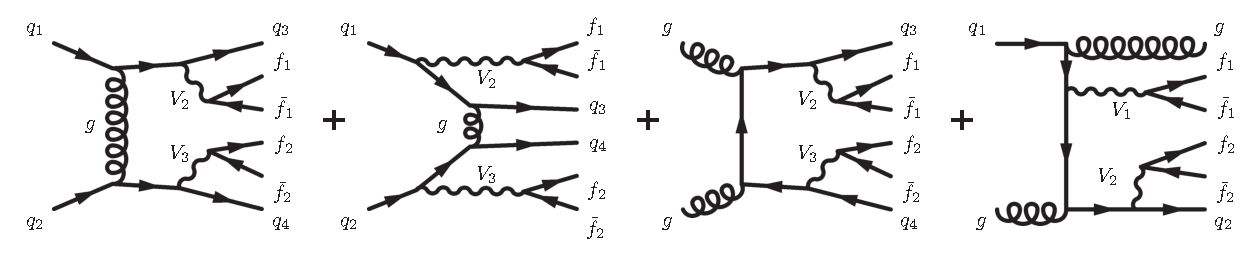
\includegraphics[width=\textwidth]{figs/ssww_13tev/diagrams/VbsQCD}
  \caption{Tree-level Feynman diagrams for QCD $VVjj$ production.  The labels are quarks ($q$), fermions ($f$), and gauge bosons ($V = W,Z$).}
  \label{fig:ssww13tev_diagrams_qcd}
\end{figure}

\subsection{Same-sign $W^{\pm}W^{\pm}$ scattering}\label{ssww13tev:ssww_topology}
Same-sign \ssww scattering is considered to be one of the best channels for studying VBS at the LHC due to its favorable ratio of EWK to QCD production~\cite{2015.higgs-constraints-from-vbs}.
Since the VBS diagrams (which are a subset of the total EWK production) are the primary source of interest for an analysis, the QCD production would be considered a background in an analysis.
Therefore a higher EWK-to-QCD ratio results in increased sensitivity to VBS.
%This is due primarily to the ratio of the EWK to the QCD production, which matters a great deal due to the VBS events being a subset of the total EWK production.
%In an analysis the EWK production would be conisdered the signal and the QCD production a background, so a favorable ratio of the two helps greatly when comparing the size of the signal to the backgrounds.
EWK and QCD cross sections at \com{13} for six leptonic $VVjj$ final states were calculated using the \tt{SHERPA} MC generator in a VBS-enriched fiducial phase space in~\cite{2014.ssww-thesis-gumpert}.
Despite its relatively low total cross section compared to some other $VVjj$ processes, the EWK-to-QCD ratio for \ssww is 10-20 times higher than for other processes after applying VBS-enhancing selection criteria.

%There are several advantages to studying the same-sign $WW$ process specifically.
%The final state's net charge of $\pm 2$ helps considerably in reducing the number of background processes that can mimic the signal.

\begin{table}[htbp]
  \centering
  \begin{tabular}{l l r r r}%S[table-format=2.3] S[table-format=2.3] S[table-format=2.3]}
    Final state & Process & $\sigma_{\textrm{EWK}}$ [fb] & $\sigma_{\textrm{QCD}}$ [fb] & $\sigma_{\textrm{EWK}}/\sigma_{\textrm{QCD}}$ \\
    \hline\hline
    $l^{\pm}l^{\mp}l^{\pm}l^{\mp} jj$ & $ZZ$                 & 0.098  & 0.100 & 0.98\\
    $l^{\pm}l^{\pm}l^{\mp}\nu jj$    & $W^{\pm}Z$            & 2.34   &  4.38 & 0.53\\
    $l^{\pm}l^{\mp}\nu\nu jj$       & $W^{\pm}W^{\mp}$, $ZZ$ & 12.3   &  21.8 & 0.56\\
    $\boldsymbol{l^{\pm}l^{\pm}\nu\nu jj}$       & \boldsymbol{$W^{\pm}W^{\pm}$}       & \bf{3.97}   & \bf{0.346} & \bf{11.47}\\
    $l^{\pm}\nu\nu\nu jj$         & $W^{\pm}Z$             & 7.64   &  15.5 & 0.49\\
    $\nu\nu\nu\nu jj$            & $ZZ$                 &  1.68  &  1.38 & 1.22 \\
    \hline
  \end{tabular}
  \caption[Predicted cross sections for EQK and QCD production of diboson processes relevant to VBS at \com{13} using the \tt{SHERPA} MC generator.  The numbers for the \ssww process are bolded. Leptons are required to have $\pt \ge 25\gev$ and lie within $|\eta| \le 2.5$ with $m_{ll} > 20\gev$, and at least two jets are required with $\pt \ge 30\gev$ and $|\eta| < 4.5$.  The VBS contributions are enhanced by requiring the dijet invariant mass $m_{jj} > 500\gev$ and dijet separation $\Delta y_{jj} > 2.4$.]{Predicted cross sections for EQK and QCD production of diboson processes relevant to VBS at \com{13} using the \tt{SHERPA} MC generator.  The numbers for the \ssww process are bolded. Leptons are required to have $\pt \ge 25\gev$ and lie within $|\eta| \le 2.5$ with $m_{ll} > 20\gev$, and at least two jets are required with $\pt \ge 30\gev$ and $|\eta| < 4.5$.  The VBS contributions are enhanced by requiring the dijet invariant mass $m_{jj} > 500\gev$ and dijet separation $\Delta y_{jj} > 2.4$.  Numbers taken from~\cite{2014.ssww-thesis-gumpert}.}
  \label{tab:ssww13tev_qcd_vs_ewk}
\end{table}

This analysis studies \ssww scattering where both $W$ bosons decay leptonically to $e\nu$ or $\mu\nu$\footnote{Throughout the rest of this chapter, unless stated otherwise, $l$ denotes either electrons ($e$) or muons ($\mu$), and $\nu$ denotes a neutrino.  Additionally, $e$, $\mu$, and $\nu$ with no charge or anti-particle designation refer interchangeably to either the particle or anti-particle.}.
The \ssww VBS final state consists of two leptons with the same electric charge, two neutrinos, and two high energy forward jets with a large invariant mass.
Tree-level Feynman diagrams of VBS \ssww production can be found in Figure~\ref{fig:ssww13tev_diagrams_vbs_ssww} and a visual representation of the VBS topology can be found in Figure~\ref{fig:ssww13tev_event_topology}.

The two tag jets in the characteristic VBS signature also serve as a powerful tool to suppress the QCD production mode.
In EWK events, the two jets tend to have much higher separation and a larger combined invariant mass than the two leading jets in a QCD event.
The two plots shown in Figure~\ref{fig:ssww13tev_dijet_comparison} highlight the differences in these dijet quantities between the two production modes.
An ATLAS event display of a real \ssww candidate event is shown in Figure~\ref{fig:ssww13tev_event_display_mm}.

% i think i really only need to include the vbs diagrams for ssww (maybe also the ewk?) since the general VV ones are above for all processes
\begin{figure}[htbp]
  \centering
  \includegraphics[width=.32\textwidth]{figs/ssww_13tev/diagrams/vbs1}
  \includegraphics[width=.32\textwidth]{figs/ssww_13tev/diagrams/vbs2}
  \includegraphics[width=.32\textwidth]{figs/ssww_13tev/diagrams/vbs3}
  \caption{Leading order Feynman diagrams for VBS EWK production of \ssww events. The leftmost diagram contains a quartic gauge coupling vertex, and the rightmost diagram contains an exchange of a Higgs boson.}
  \label{fig:ssww13tev_diagrams_vbs_ssww}
\end{figure}

\begin{figure}[htbp]
  \centering
  \includegraphics[width=.95\textwidth]{figs/ssww_13tev/introduction/vbs_event_topology}
  \caption{\ssww VBS event topology containing two leptons (1 and 2) with the same electric charge, two neutrinos, and two forward tagging jets (3 and 4) with large rapidity separation $\Delta y$.}
  \label{fig:ssww13tev_event_topology}
\end{figure}

\begin{figure}[htbp]
  \centering
  \begin{subfigure}[b]{.48\textwidth}
    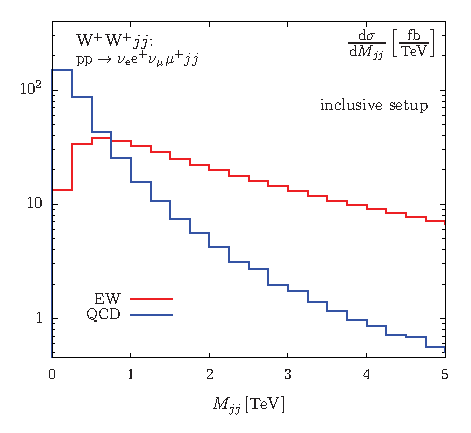
\includegraphics[width=\textwidth]{figs/ssww_13tev/introduction/vbs_mjj}
    \caption{Dijet invariant mass}
    \label{fig:ssww13tev_dijet_comparison_mjj}
  \end{subfigure}
  \begin{subfigure}[b]{.4842\textwidth}
    \includegraphics[width=\textwidth]{figs/ssww_13tev/introduction/vbs_dyjj}
    \caption{Dijet separation}
    \label{fig:ssww13tev_dijet_comparison_dyjj}
  \end{subfigure}
  \caption[Generator level comparisons at \com{7} of dijet invariant mass ($m_{jj}$, left) and dijet rapidity ($\Delta y_{jj}$, right) in EWK (red) and QCD (blue) \ssww events with no selection cuts applied.]{Generator level comparisons at \com{7} of dijet invariant mass ($m_{jj}$, left) and dijet rapidity ($\Delta y_{jj}$, right) in EWK (red) and QCD (blue) \ssww events with no selection cuts applied.  Plots taken from~\cite{2017.physics-opportunities-100tev}.}
  \label{fig:ssww13tev_dijet_comparison}
\end{figure}

\begin{figure}[htbp]
  \centering
  \includegraphics[width=.95\textwidth]{figs/ssww_13tev/introduction/evtdisplay_mm}
  \caption[ATLAS event display of a $pp\rightarrow W^{+}W^{+}\rightarrow\mu^{+}\nu_\mu\mu^{+}\nu_\mu jj$ event.  The muons are represented by the red lines travelling from the ID through the MS, and the forward jets are represented by the blue cones with yellow energy deposits in the calorimeters.  The direction of the $\met$ in the transverse plane is indicated by the gray dashed line in the inset image.]{ATLAS event display of a $pp\rightarrow W^{+}W^{+}\rightarrow\mu^{+}\nu_\mu\mu^{+}\nu_\mu jj$ event.  The muons are represented by the red lines travelling from the ID through the MS, and the forward jets are represented by the blue cones with yellow energy deposits in the calorimeters.  The direction of the $\met$ in the transverse plane is indicated by the gray dashed line in the inset image.  Event display taken from~\cite{2018.ssww-13tev-atlas-conf}.}
  \label{fig:ssww13tev_event_display_mm}
\end{figure}

\subsection{Overview of backgrounds}\label{ssww13tev:background_overview}
In addition to QCD production of \ssww events, there are several other processes that can end up with a final state of two same-sign leptons, two neutrinos, and two jets.
However, due to the $\pm 2$ final state charge, there is a considerable reduction in SM backgrounds (such as $Z$ boson events) when compared to an analysis like opposite-sign \oswwjj.

One of the largest sources of background involves processes with prompt leptons\footnote{Prompt leptons are those that are produced in the primary collision and are a direct decay product of the process of interest.  Non-prompt leptons originate from some secondary process, such as a $b$-hadron decay, or are jets that get mis-reconstructed as a lepton.}.
These are events that contain two leptons with the same electric charge and one or more additional leptons that are ``lost'', either by failing the selection criteria or falling outside of the detector's acceptance.
The number of processes that can contribute is limited by the requirement of same-sign leptons, and as a result this background is dominated by processes involving two or more vector bosons, with the largest contribution coming from $WZ$ events and smaller contributions from $ZZ$ and $t\bar{t}+V$ events.
Triboson events where one boson decays hadronically also contribute to this background; however, the jets are generally softer and more central than in a typical VBS event, and the cuts applied on the forward jets suppress these contributions.

The other dominant background comes from non-prompt, or ``fake'', leptons.
Here one or more leptons originate from the decay of another particle unrelated to the signal process, such as a heavy-flavor decay or photon conversion, or come from a jet that is misidentified as a lepton.
This background is mostly made up of events from $t\bar{t}$ and $W$+jets processes, with a much smaller contribution from conversions in $V\gamma$ events. %\TODO{check whether $V\gamma$ really qualifies as non-prompt, we lump $Z\gamma$ in with the charge flip background in the paper...}

Finally, opposite-sign lepton pairs can enter the signal region if one of the leptons is reconstructed with the wrong charge (called \emph{charge misidentification}\footnote{Charge misidentification is also referred to interchangeably as \emph{charge mis-ID} and \emph{charge flip}.}).
In practice, this only affects events with electrons, as the charge misidentification rate for muons is negligible~\cite{2013.muon-flip}.
This is a major background in events with two electrons, but is a much smaller contribution for events with one electron and one muon.

%\subsection{}\label{ssww13tev:theory}
%The theoretical motivation for studying the ssWW process is detailed in Section~\ref{ssww13tev:vbs_theory}.
\TODO{Re-write this section referencing the main description in the 13tev section. Maybe just turn this into a 1 or 2 sentence refresher}
The particular interest in polarization is the potential for the scattering amplitude of longitudinally polarized weak bosons to diverge linearly as the center of mass energy increases, ultimately violating unitarity around $1\tev$ \cite{1977.ben-lee-weak-interactions}.
In the Standard Model, the Higgs boson cancels these divergences.
However, as the Higgs is recently discovered it is still extremely to study the mechanism of electroweak symmetry breaking (EWSB), and the longitudinal scattering of $W$ bosons is expected to be one of the most sensitive tests of EWSB~\cite{2013.longitudinal-theory}.

%some additional detail on the interest in the longitudinally polarized $W$ bosons follows \cite{2016.ssww-polarization, 2013.longitudinal-theory, 2017.multiboson-at-lhc}.

\subsection{Experimental sensitivity to longitudinal polarization}\label{sec:sswwupgrade_longitudinal_sens}
\TODO{mention that since there are so many polarization possibilities, a large integrated luminosity is needed to measure just one of them individually}
There are three possible polarization states for a massive vector boson: two transverse ($+$ or $-$) and one longitudinal ($0$).
Therefore, in a system with two $W$ bosons, the overall polarization can be purely longitudinal ($00$), purely transverse ($++$, $--$, and $+-$), or mixed ($+0$ and $-0$).
The three combinations will be referred to as \emph{LL}, \emph{TT}, and \emph{LT} respectively.

In order extract the longitudinal scattering component, it is necessary to find variables that distinguish the LL from the TT and LT.
Several variables were studied, and those with the best discriminating power between the polarizations were the leading and subleading lepton $\pt$ as well as the azimuthal separation ($|\dphijj|$) of the two VBS jets.
The LL events preferred lower $\pt$ for both signal leptons (see Figure~\ref{fig:polarization_leppt}), which motivates keeping these two cuts as low as possible in the event selection in order to preserve as much longitudinal polarization as possible.
In the case of $|\dphijj|$, the LL events generally had a larger dijet separation (see Figure~\ref{fig:polarization_dphijj}), and this variable is used in a binned likelihood fit to extract the longitudinal scattering significance.

\begin{figure}[htp]
  \centering
  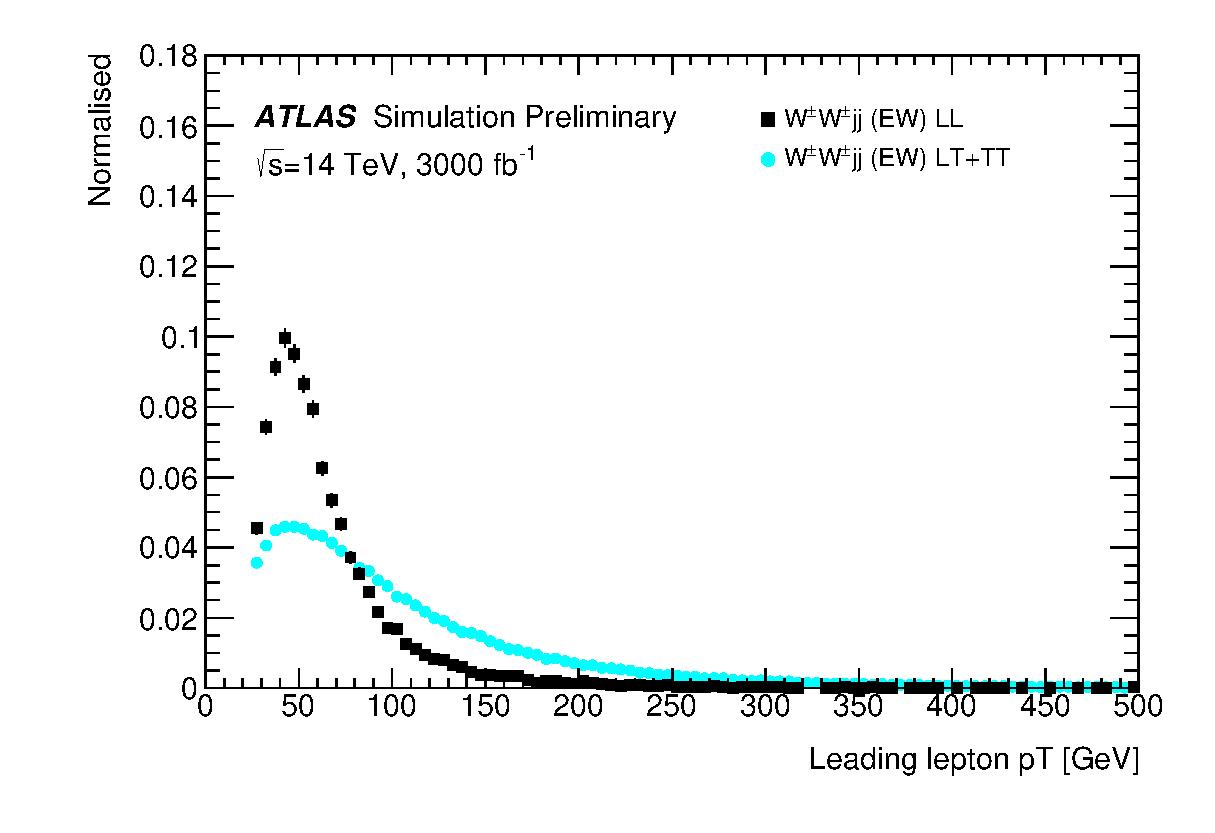
\includegraphics[width=0.8\textwidth]{figs/ssww_upgrade/polarization/lepton0_pt_pass9}\\
  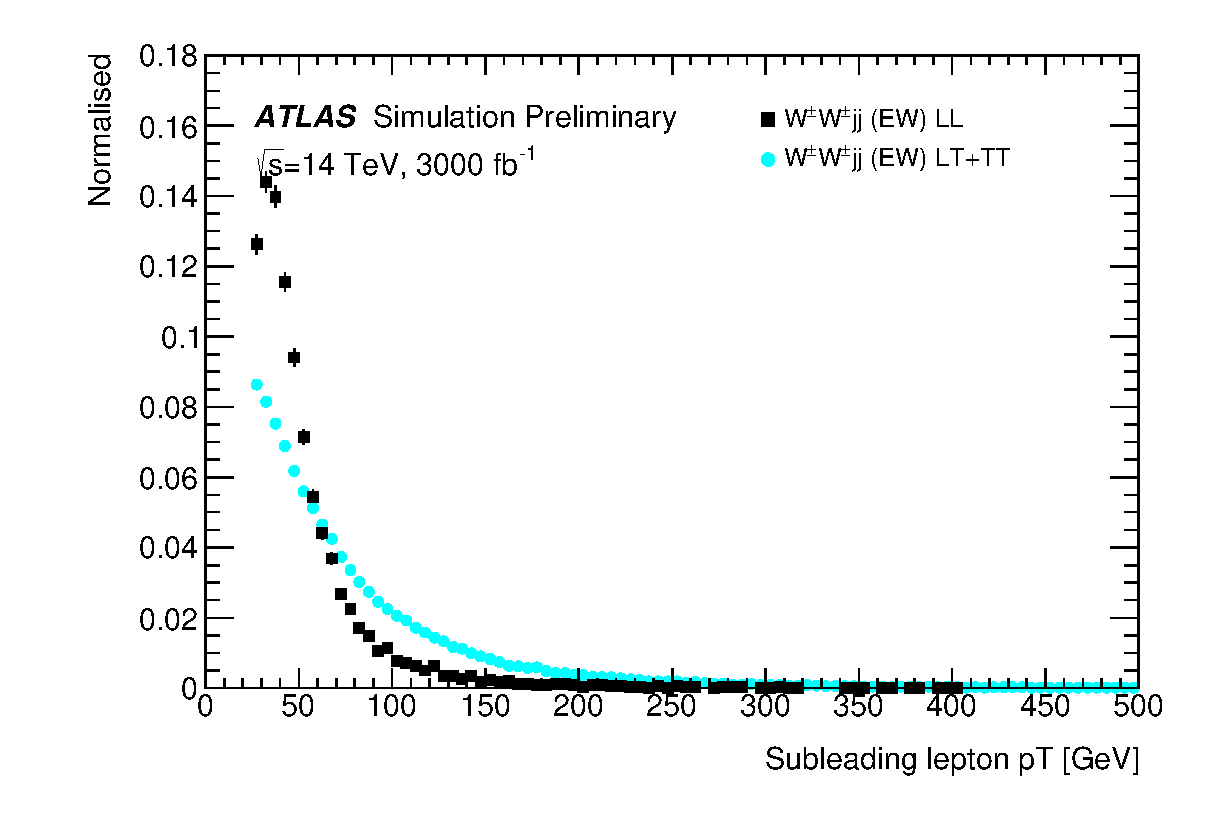
\includegraphics[width=0.8\textwidth]{figs/ssww_upgrade/polarization/lepton1_pt_pass9}
  \caption{Comparison of the leading (top) and subleading (bottom) lepton $\pt$ distributions for purely longitudinal (LL, black) and mixed polarization (LT+TT, cyan) \ssww events.}
  \label{fig:polarization_leppt}
\end{figure}

\begin{figure}[htp]
  \centering
  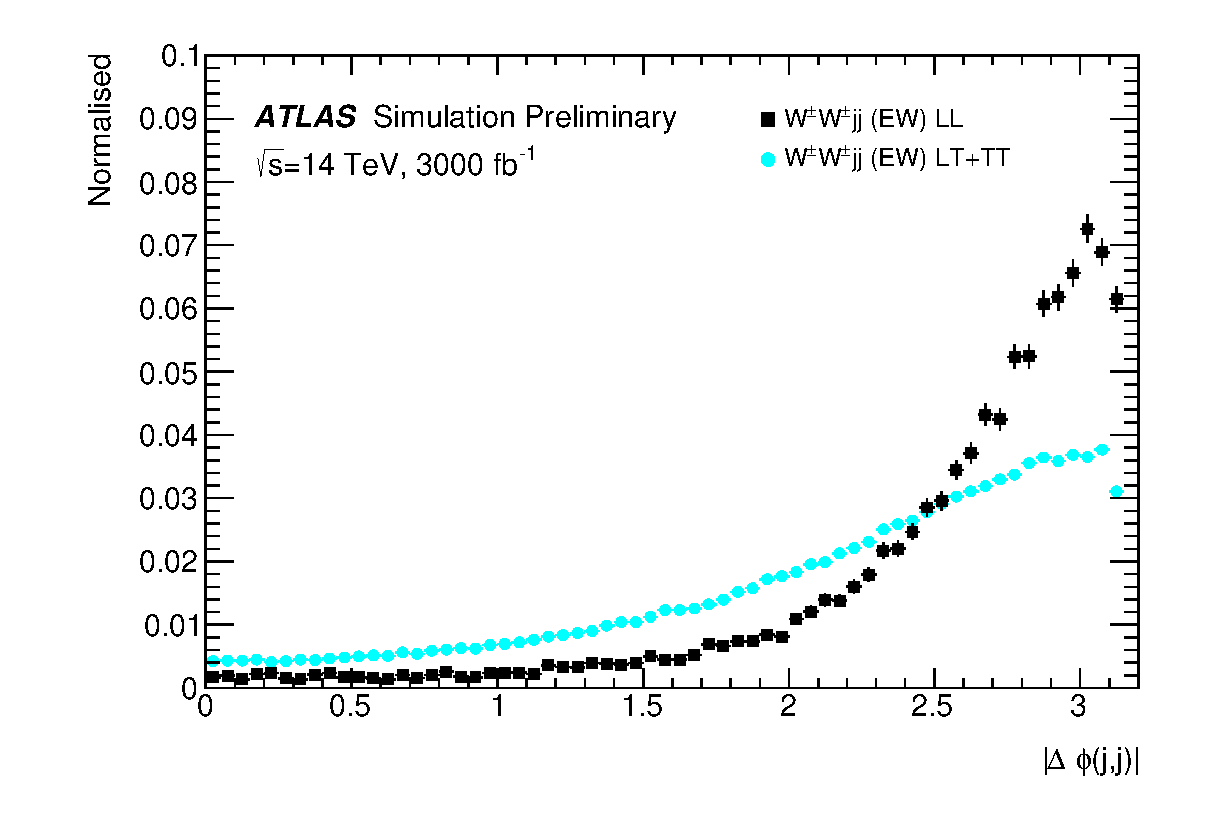
\includegraphics[width=0.8\textwidth]{figs/ssww_upgrade/polarization/dijet_absdphijj_pass9}
  \caption{Comparison of the azimuthal dijet separation ($|\dphijj|$) for purely longitudinal (LL, black) and mixed polarization (LT+TT, cyan) \ssww events.}
  \label{fig:polarization_dphijj}
\end{figure}



%\section{Theoretical motivation}\label{ssww13tev:theory}
%The theoretical motivation for studying the ssWW process is detailed in Section~\ref{ssww13tev:vbs_theory}.
\TODO{Re-write this section referencing the main description in the 13tev section. Maybe just turn this into a 1 or 2 sentence refresher}
The particular interest in polarization is the potential for the scattering amplitude of longitudinally polarized weak bosons to diverge linearly as the center of mass energy increases, ultimately violating unitarity around $1\tev$ \cite{1977.ben-lee-weak-interactions}.
In the Standard Model, the Higgs boson cancels these divergences.
However, as the Higgs is recently discovered it is still extremely to study the mechanism of electroweak symmetry breaking (EWSB), and the longitudinal scattering of $W$ bosons is expected to be one of the most sensitive tests of EWSB~\cite{2013.longitudinal-theory}.

%some additional detail on the interest in the longitudinally polarized $W$ bosons follows \cite{2016.ssww-polarization, 2013.longitudinal-theory, 2017.multiboson-at-lhc}.

\subsection{Experimental sensitivity to longitudinal polarization}\label{sec:sswwupgrade_longitudinal_sens}
\TODO{mention that since there are so many polarization possibilities, a large integrated luminosity is needed to measure just one of them individually}
There are three possible polarization states for a massive vector boson: two transverse ($+$ or $-$) and one longitudinal ($0$).
Therefore, in a system with two $W$ bosons, the overall polarization can be purely longitudinal ($00$), purely transverse ($++$, $--$, and $+-$), or mixed ($+0$ and $-0$).
The three combinations will be referred to as \emph{LL}, \emph{TT}, and \emph{LT} respectively.

In order extract the longitudinal scattering component, it is necessary to find variables that distinguish the LL from the TT and LT.
Several variables were studied, and those with the best discriminating power between the polarizations were the leading and subleading lepton $\pt$ as well as the azimuthal separation ($|\dphijj|$) of the two VBS jets.
The LL events preferred lower $\pt$ for both signal leptons (see Figure~\ref{fig:polarization_leppt}), which motivates keeping these two cuts as low as possible in the event selection in order to preserve as much longitudinal polarization as possible.
In the case of $|\dphijj|$, the LL events generally had a larger dijet separation (see Figure~\ref{fig:polarization_dphijj}), and this variable is used in a binned likelihood fit to extract the longitudinal scattering significance.

\begin{figure}[htp]
  \centering
  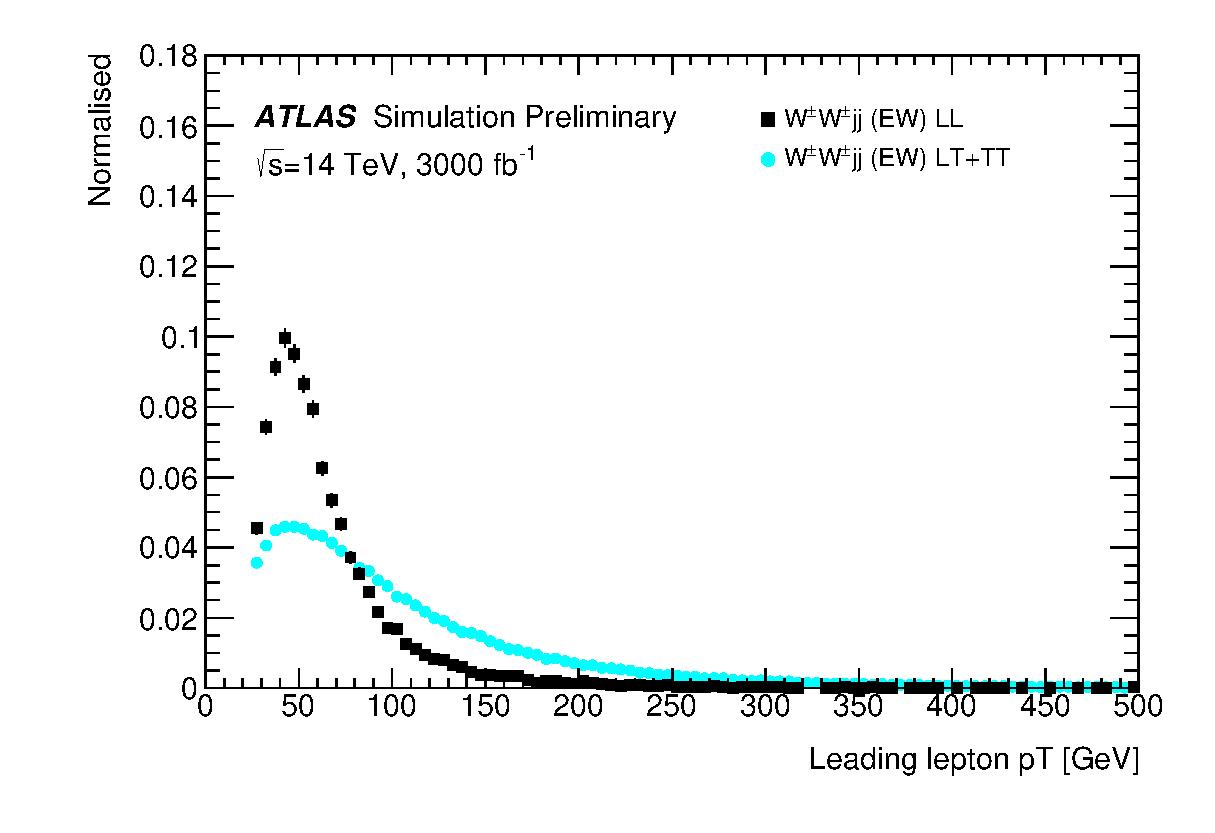
\includegraphics[width=0.8\textwidth]{figs/ssww_upgrade/polarization/lepton0_pt_pass9}\\
  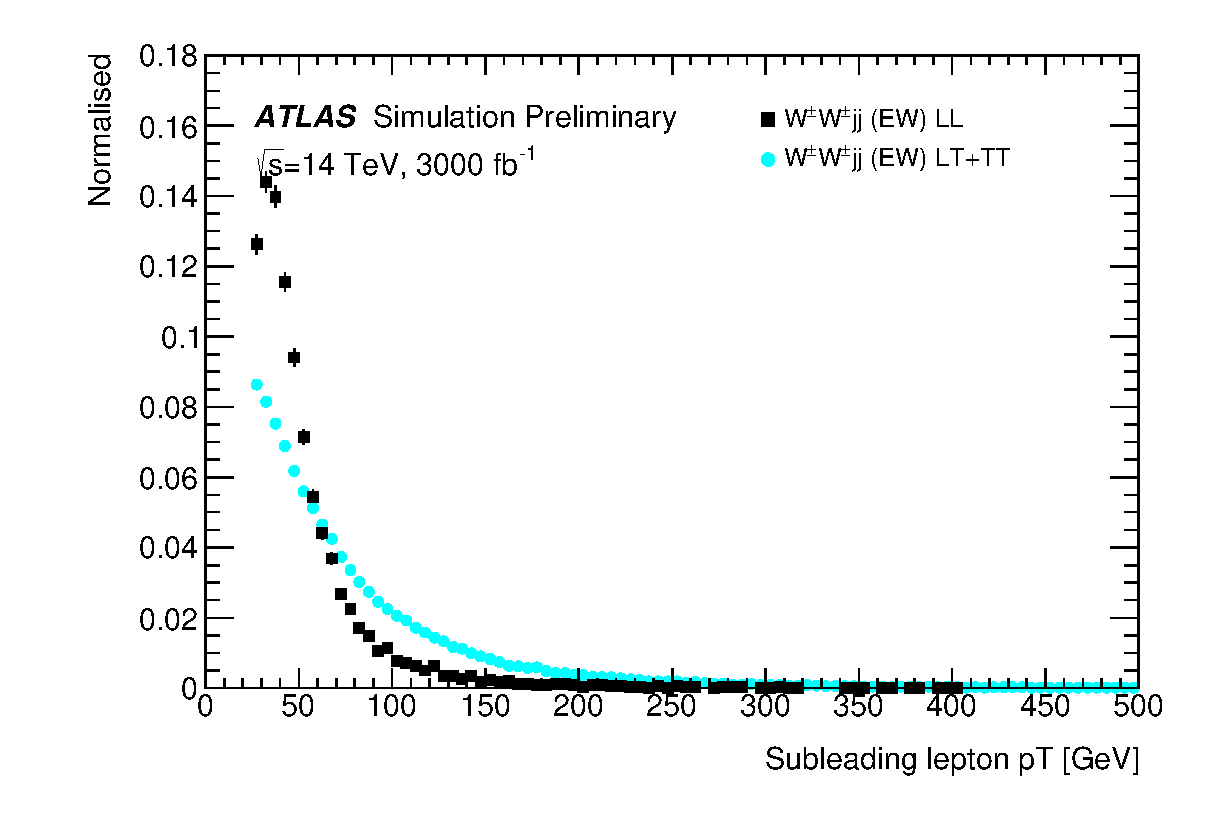
\includegraphics[width=0.8\textwidth]{figs/ssww_upgrade/polarization/lepton1_pt_pass9}
  \caption{Comparison of the leading (top) and subleading (bottom) lepton $\pt$ distributions for purely longitudinal (LL, black) and mixed polarization (LT+TT, cyan) \ssww events.}
  \label{fig:polarization_leppt}
\end{figure}

\begin{figure}[htp]
  \centering
  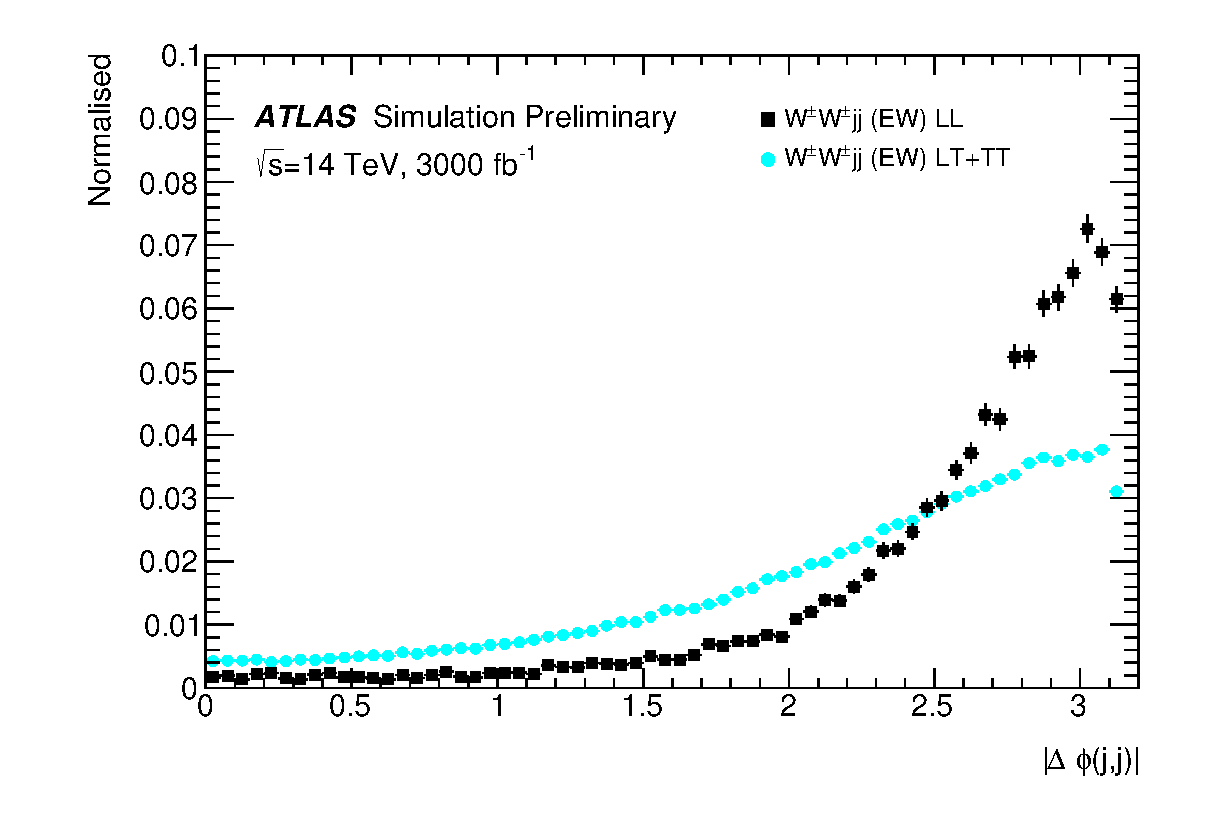
\includegraphics[width=0.8\textwidth]{figs/ssww_upgrade/polarization/dijet_absdphijj_pass9}
  \caption{Comparison of the azimuthal dijet separation ($|\dphijj|$) for purely longitudinal (LL, black) and mixed polarization (LT+TT, cyan) \ssww events.}
  \label{fig:polarization_dphijj}
\end{figure}


\section{Data and Monte Carlo samples}\label{ssww13tev:data_mc}
\subsection{Data samples}\label{ssww13tev:data}

\subsection{Monte Carlo samples}\label{ssww13tev:mc}


\section{Object and event selection}\label{ssww13tev:object_event_selection}
\subsection{Object selection}

\subsection{Event selection}


%\section{Signal definition}\label{ssww13tev:signal}
%Hello world!

\subsection{Sensitivity to longitudinal polarization}


\section{Background estimations}\label{ssww13tev:background}
The major sources of background events are summarized in Section~\ref{ssww13tev:background_overview}, and the methods used to estimate them are detailed in this section.  
Prompt backgrounds from $ZZ$ and $t\bar{t}V$ are estimated directly from MC simulations.
The shape of the $WZ$ and $V\gamma$ backgrounds are taken from MC, and the predicted yeilds are normalized to the data predictions in dedicated control regions, as outlined in Sections~\ref{ssww13tev:wz} and \ref{ssww13tev:wgamma}, respectively.
Opposite sign events with a charge misidentified electron are estimated by a data-driven background method which is summarized in Section~\ref{ssww13tev:charge_misid}.
Finally, a \emph{fake factor} method is used to estimate the contributions from non-prompt backgrounds and is the subject of Section~\ref{ssww13tev:fake_factor}.

\subsection{Estimation of the $WZ$ background}\label{ssww13tev:wz}
The dominant background involving prompt leptons comes from $WZ$+jets events.
The contribution is estimated from MC simulation and normalized to data in a control region enriched in $WZ$ events defined by the same event selection as Table~\ref{tab:ssww13tev_event_selection} for the signal region, with the following changes applied to increase the purity of the $WZ$ process:
\begin{itemize}
\item The third lepton veto is inverted, requiring a third lepton with $\pt > 15\gev$
\item Two of the leptons must make a same-flavor opposite-sign pair. If more than one pair exists, the one with $m_{ll}$ closest to the $Z$ boson mass is chosen.
\item The trilepton invariant mass is required to be $m_{lll} > 106\gev$ to reduce contributions from $Z\gamma$ and $Z$+jets
\end{itemize}

Once the event yields in the control region are calculated, they are propagated to the final signal region fit, detailed in Section~\ref{ssww13tev:xsec} \TODO{update reference with proper subsection once it's written}, in a single bin combining all the lepton channels.
The systematic uncertainties of the $WZ$ background are also calculated at this time.
The event yields for the $WZ$ control region are listed in Table~\ref{tab:ssww13tev_wzcr_yields}, and distributions of the leading lepton $\pt$ and $\eta$ as well as trilepton invariant mass $m_{lll}$ are found in Figures~\ref{fig:ssww13tev_wzcr_lep0} and \ref{fig:ssww13tev_wzcr_mlll}, respectively.

\begin{table}[htbp]
  \centering
  \begin{tabular}{l r}
    \multicolumn{2}{c}{Event yields in the $WZ$ control region} \\
    \hline\hline
    $WZ$     & $197.9\pm 1.4$ \\
    $ZZ$     & $14.1\pm 0.3$ \\
    Triboson & $1.26\pm 0.1$ \\
    top      & $10.8\pm 1.1$ \\
    $Z\gamma$& $3.1\pm 1.1$ \\
    $Z$+jets & $2.5\pm 1.4$ \\
    \hline
    Total prediction & $229.7\pm 2.5$ \\
    Data             & $201 \pm 14.2$ \\
    \hline
  \end{tabular}
  \caption{Event yields in the $WZ$ control region before normalization.  All lepton flavor channels are combined.}
  \label{tab:ssww13tev_wzcr_yields}
\end{table}

\begin{figure}[htbp]
  \centering
  \includegraphics[width=.48\textwidth]{figs/ssww_13tev/backgrounds/wz/ll-CutCRWZ3Lep-l0_pt-lin}
  \includegraphics[width=.48\textwidth]{figs/ssww_13tev/backgrounds/wz/ll-CutCRWZ3Lep-l0_eta-lin}
  \caption{Leading lepton $\pt$ (left) and $\eta$ (right) distributions in the $WZ$ control region before normalization.  All lepton channels are combined.}
  \label{fig:ssww13tev_wzcr_mlll}
\end{figure}

\begin{figure}[htbp]
  \centering
  \includegraphics[width=.48\textwidth]{figs/ssww_13tev/backgrounds/wz/ll-CutCRWZ3Lep-Mlll-lin}
  \caption{Trilepton invariant mass $m_{lll}$ distribution in the $WZ$ control region before normalization.  All lepton channels are combined.}
  \label{fig:ssww13tev_wzcr_lep0}
\end{figure}

\subsection{Estimation of the $V\gamma$ background}\label{ssww13tev:wgamma}
Events from $V\gamma$ processes can pass selection if the photon converts into an $e^{+}e^{-}$ pair and one of the electrons passes the selection criteria.
The background is estimated from MC simulations which are then scaled by a normalization factor calculated from a control region enriched in $Z(\mu^{+}\mu^{-})\gamma$ events.
This control region selects two opposite-sign muons and an additional electron that is assumed to come from the photon conversion.
The full event selection is detailed in Table~\ref{tab:ssww13tev_vgamma_cr}.

\begin{table}[htbp]
  \centering
  \begin{tabular}{c}
    $V\gamma$ control region \\
    \hline\hline
    Exactly two muons with $\pt > 27\gev$ and $\pt > 20\gev$ \\
    Exactly one additional electron with $\pt > 15\gev$ \\
    Remove overlap between $Z$+jets and $Z\gamma$ \\
    Di-muon + photon invariant mass $75 < M_{\mu\mu\gamma} < 100\gev$ \\
    $\met < 30\gev$ \\
    \hline
  \end{tabular}
  \caption{Selection criteria for the $V\gamma$ control region.}
  \label{tab:ssww13tev_vgamma_cr}
\end{table}

The $Z\gamma$ MC samples available do not cover the full range of $\pt^\gamma$ and $\deltar(\gamma,l)$; thus, additional Drell-Yan samples ($Z$+jets) are used to fill out the phase space.
Overlap between the two samples are removed based to avoid double counting.
Events with final state photons at truth level are checked to ensure that the photon did not originate from a hadronic decay.
Cuts on $\pt^\gamma > 10\gev$ and $\deltar(\gamma,l) > 0.1$ are then applied at generator level, and $Z\gamma$ events that fail and $Z$+jets events that pass this additional selection are removed.

The normalization factor is calculated directly from the event yields in the $V\gamma$ control region rather than in the signal fit, as is done for the $WZ$ background.
The event yields are listed in Table~\ref{tab:ssww13tev_vgamma_numbers}, and the normalization factor is determined to be $1.77$.
No MC events from $Z\gamma$ processes survive the full event selection; thus, the scaling is only applied to the $W\gamma$ background in the signal region.
A systematic uncertainty of 44\% is assigned to the background based off of the uncertainties in the calculation of the normalization factor.

\begin{table}[htbp]
  \centering
  \begin{tabular}{l r}
    \multicolumn{2}{c}{Event yields in the $V\gamma$ control region} \\
    \hline\hline
    $Z\gamma$ & $24.6\pm 3.3$ \\
    $Z$+jets  &  $3.0\pm 1.5$ \\
    diboson + triboson & $6.7\pm 0.3$ \\
    top       &  $1.5\pm 0.5$ \\
    \hline
    Total prediction & $35.8\pm 3.7$ \\
    Data             & $57 \pm 7.6$ \\
    %\hline
    %Data - prediction & $21.2\pm 8.4$ \\
    \hline
  \end{tabular}
  \caption{Event yields in the $V\gamma$ control region.  The $V\gamma$ scale factor of 1.77 is calculated by scaling up the $Z\gamma$ and $Z$+jets backgrounds to account for the difference between the data and predicted total background.}
  \label{tab:ssww13tev_vgamma_numbers}
\end{table}

\subsection{Estimation of backgrounds from charge misidentification}\label{ssww13tev:charge_misid}
If an electron's charge is mis-reconstructed, it can lead to a real, opposite-sign lepton pair passing the same-sign requirement in the event selection.
There are two primary reasons this can occur:
\begin{enumerate}
\item An electron emits a photon via bremsstrahlung which then converts into an electron-positron pair, and the conversion track with the wrong electric charge is matched to the original electron.
This is the dominant process leading to charge flip, and it is highly dependent on the electron $\eta$ due to the different amount of detector material the electron passes through.
\item The curvature of the electron's track is mismeasured, resulting in the wrong charge being assigned.
This process is dependent on the momentum of the electron, as its track becomes more straight as the momentum of the electron increases.
\end{enumerate}

In order to estimate this background, the rate at which an electron's charge is misidentified is calculated from $Z\rightarrow e^{+}e^{-}$ MC simulation.
It is known that the MC does not perfectly model the material effects leading to charge flip; as a result, scale factors are applied to the MC in order for it to to better reflect the real performance.
These scale factors are obtained from the ratio of charge mis-ID rates in data and uncorrected MC in~\cite{2018.ssww-13tev-atlas-support} following the method outlined in~\cite{2017.charge-flip-support}.
Once the scale factors are applied, the charge misidentification rate $\varepsilon$ can be extracted by comparing the electron's reconstructed charge with the charge of its truth particle:
\begin{equation}
  \varepsilon(\eta,\pt) = \frac{N_{\textrm{wrong\ charge}}}{N_{\textrm{prompt\ electrons}}}
\end{equation}
The charge mis-ID rate is calculated in bins of electron $|\eta|$ and $\pt$ and varies from below $0.1\%$ in the central region of the detector up to $8\%$ in the forward regions for high $\pt$ (above $90\gev$) electrons.
A two-dimensional plot of $\varepsilon$ can be found in Figure~\ref{fig:charge_flip_rates}.

\begin{figure}
  \centering
  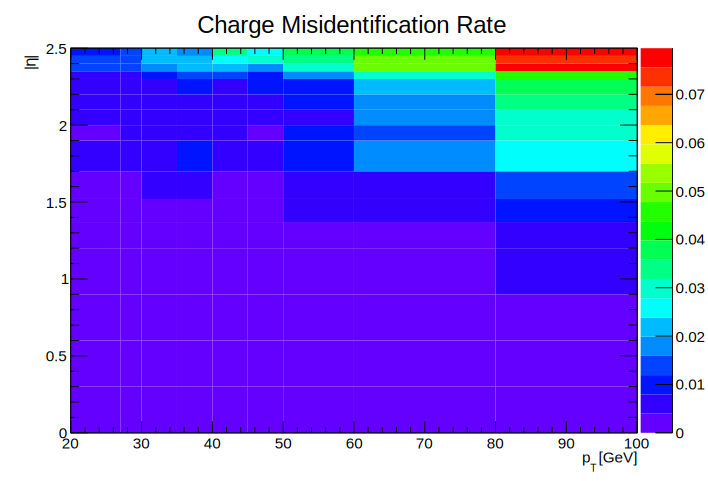
\includegraphics[width=.7\textwidth]{figs/ssww_13tev/backgrounds/charge_flip/charge_flip_2d}
  \caption{Charge misidentification rates for electrons as a function of $|\eta|$ and $\pt$.  Rates are calculated from $Z\rightarrow e^{+}e^{-}$ MC after applying sacle factors to approximate the charge mis-ID rates in data.}
  \label{fig:charge_flip_rates}
\end{figure}

%The size of the charge mis-ID background in a given region (signal or control region) is estimated from events that pass the region's default event selection but with an opposite-sign lepton pair.
Given the charge flip rate $\varepsilon(\eta,\pt)$, the rate at which an electron has its charge correctly reconstructed is $(1-\varepsilon)$.
Thus there are three possible combinations of charge identification, assuming a two-electron event:
\begin{enumerate}
\item Both electrons are reconstructed correctly: $(1-\varepsilon)^2$
\item Both electrons are mis-reconstructed: $\varepsilon^2$
\item Only one electron is mis-reconstructed: $2\varepsilon(1-\varepsilon)$
\end{enumerate}

In order to estimate the size of the background from charge misidentification, opposite-sign events are selected using the default event selection for a given signal or control region with the same-sign requirement inverted.
These events are then weighted by the probability for one of the electrons to be reconstructed with the wrong charge:
\begin{equation}
\omega = \frac{\varepsilon_1(1-\varepsilon_2)+\varepsilon_2(1-\varepsilon_1)}{(1-\varepsilon_1)(1-\varepsilon_2)+\varepsilon_1\varepsilon_2}
\label{ssww13tev:ch_flip_weight}
\end{equation}
%\begin{equation}
%\omega = \frac{\varepsilon_1(1-\varepsilon_2)+\varepsilon_2(1-\varepsilon_1)}{1-(\varepsilon_1+\varepsilon_2)+2\varepsilon_1\varepsilon_2}
%\label{ssww13tev:ch_flip_weight2}
%\end{equation}
where the subscripts 1 and 2 refer to the leading and subleading electrons, respectively, and $\varepsilon_i$ is a function of the $\eta$ and $\pt$ of the $i^{\textrm{th}}$ electron.
In the case of an event with only one electron and one muon, Equation~\ref{ssww13tev:ch_flip_weight} simplifies:
\begin{equation}
\omega = \frac{\varepsilon}{1-\varepsilon}
\end{equation}
This method assumes that there is little contamination from fake electrons in the opposite-sign sample, and this has been verified with MC simulation.

Additionally, charge-flipped electrons tend to be reconstructed with lower energy when compared to electrons with the correct charge.
This is due to energy loss from the material interactions that can cause the charge to be misidentified.
A correction factor is calculated from MC simulations, comparing the $\pt$ of the truth electron to its reconstructed counterpart:
\begin{equation}
\alpha = \frac{\Big(\frac{\pt^{\textrm{reco}}}{\pt^{\textrm{truth}}}-1\Big)_{\textrm{correct charge}}}{\Big(\frac{\pt^{\textrm{reco}}}{\pt^{\textrm{truth}}}-1\Big)_{\textrm{wrong charge}}}
\label{ssww13tev:ch_flip_alpha}
\end{equation}
The correction is then applied to the $\pt$ of the charge-flipped electron via
\begin{equation}
\pt = \pt^0/(1+\alpha)+dE
\label{ssww13tev:ch_flip_energy_corr}
\end{equation}
where $\pt^0$ is the uncorrected $\pt$ of the electron and $dE$ is a gaussian smearing factor centered at zero with a width related to the energy resolution.
Since which electron is misreconstructed is never determined in this method, in the case of a two-electron event, the energy correction is applied randomly to one of the two electrons based on the probabilities for them to be charge-flipped.
This also determines the overall sign of the event; the charge of the electron that does not recieve the correction is taken to be the charge for both.

Systematic uncertainties on the charge mis-ID rates are calculated by generating two additional sets of rates with the uncertainties on the scale factors varied up and down.
The size of the estimated charge flip background without the energy correction applied is also taken as a systematic uncertainty.
These systematic uncertainties are estimated to be approximately $\pm 15\%$.

\subsubsection{Validation of the charge misidentification estimate}\label{ssww13tev:ssincl_vr}
%The performance of the charge misidentification estimation is tested in $e^{\pm}e^{\pm}$ events with a di-electron invariant mass that lies within $15\gev$ of the $Z$ boson mass.
%Disagreements between data and background at high $\pt$ and $\eta$ have been found to be due to backgrounds from misidentified leptons, which are not included due to unreliable modeling in this particular region.

The performance of the charge misidentification estimation is tested in the same-sign inclusive validation region (VR), defined in Table~\ref{tab:ssww13tev_ssincl_vr_def}.
For $ee$ events, the mass of the dilepton pair is required to lie within $15\gev$ of the $Z$ boson mass to increase the purity of the charge flip background.
$t\bar{t}$ production, which can contribute to both the charge mis-ID and fake lepton backgrounds, is suppressed by the $b$-jet veto.
The di-electron invariant mass is shown in Figure~\ref{fig:ssww13tev_ssincl_mll}, and distributions of the leading and subleading electron $\pt$ in the $ee$-channel are shown in Figure~\ref{fig:ssww13tev_ssincl_ptlep} with the $Z$ mass cut inverted.
Agreement between data and prediction is seen within the total statistical and systematic uncertainties in the VR.

\begin{table}[htbp]
  \centering
  \begin{tabular}{c}
    Same-sign inclusive VR \\
    \hline\hline
    Exactly 2 same-sign signal leptons\\
    $\pt > 27\gev$ for both leptons \\
    $m_{ll} > 20\gev$\\
    $|m_{ee} - m_Z| > 15\gev$ ($\ee$-channel only) \\
    $N_{b\textrm{-jet}} = 0$\\
    \hline
  \end{tabular}
  \caption{Selection criteria for the same-sign inclusive validation region.}
  \label{tab:ssww13tev_ssincl_vr_def}
\end{table}

\begin{figure}
  \centering
  \includegraphics[width=.48\textwidth]{figs/ssww_13tev/backgrounds/charge_flip/ee-CutCRInclusiveSSZ-Mll_Zpeak-lin}
  \caption{Dilepton invariant mass distribution $m_{ll}$ for the $ee$ channel in the same-sign inclusive VR.}
  \label{fig:ssww13tev_ssincl_mll}
\end{figure}

\begin{figure}
  \centering
  \includegraphics[width=.48\textwidth]{figs/ssww_13tev/backgrounds/charge_flip/ee-CutCRInclusiveSSZVeto-l0_pt-lin.pdf}
  \includegraphics[width=.48\textwidth]{figs/ssww_13tev/backgrounds/charge_flip/ee-CutCRInclusiveSSZVeto-l1_pt-lin.pdf}
  \caption{$\pt$ distributions for the leading (left) and subleading (right) electron for the $ee$ channel in the same-sign inclusive VR.  In these plots, the cut requiring $m_{ee}$ to fall within the $Z$ mass window has been inverted in order to test the modelling away from the $Z$ peak.}
  \label{fig:ssww13tev_ssincl_ptlep}
\end{figure}

\subsection{Estimation of non-prompt backgrounds with the fake factor method}\label{ssww13tev:fake_factor}
Events with one prompt lepton produced in asociation with hadronic jets can pass the event selection if a jet is misidentified as a charged lepton or if a non-prompt lepton from the decay of a heavy flavor particle (such as $b$- and $c$-hadrons) passes the signal lepton criteria.
These misidentified jets and non-prompt leptons are collectively referred to as \emph{fake leptons}, or simply \emph{fakes}.
The rate at which a fake lepton is misidentified is generally not modelled well enough by the MC to accurately estimate their contributions directly from simulation.
Therefore, a data-driven technique called the \emph{fake factor} is used to estimate the size and shape of background processes from fake leptons.
In this analysis, a new modification to the fake factor is used involving the particle isolation variables; the method is outlined in the context of the \emph{default} fake factor in Section~\ref{ssww13tev:ff_method_default}, and the modified fake factor is outlined in Section~\ref{ssww13tev:ff_method_ptcone}.

%---------------------------------------------------------------------------------------------
%
%---------------------------------------------------------------------------------------------
\subsubsection{Overview of the default fake factor method}\label{ssww13tev:ff_method_default}
The goal of the fake factor method is to measure the fake rate from real collision events in a region enriched in fake leptons and use it to estimate the size of the fake lepton background in a chosen signal or control region.
This is done by creating two samples using different lepton definitions: 
\begin{enumerate}
\item The \emph{nominal} sample is made up of leptons passing the signal selection.
\item The \emph{loose} sample is made up of leptons that fail the signal selection while still passing a loosened set of criteria.  This sample is enriched in fake leptons and is orthogonal to the set of signal leptons.
\end{enumerate}
Using the sets of nominal and loose leptons, a fake factor $f$ can be calculated in a region enriched in processes that are prone to producing fake leptons:
\begin{equation}
f = \frac{N_{\textrm{nominal}}}{N_{\textrm{loose}}}
\label{eq:ssww13tev_ff_default_unbinned}
\end{equation}
Since the fake rate is not expected to be constant over the entire phase space, the fake factor can be divided into bins:
\begin{equation}
f(b) = \frac{N_{\textrm{nominal}}(b)}{N_{\textrm{loose}}(b)}
\label{eq:ssww13tev_ff_default_binned}
\end{equation}
where $b$ represents the bin number.
In this analysis, the fake factor is binned in lepton $\pt$.

In order to estimate the fake background contribution in a given signal or control region, the fake factor is applied to a second control region with a selection identical to the region of interest with one of the leptons required to satisfy the loose criteria.
The region for which the background is estimated contains two nominal leptons and is referred to as \emph{nominal+nominal} ($NN$), and the associated control region where the fake factor is applied contains one nominal and one loose lepton and is referred to as \emph{nominal+loose} ($NL$).
The fake background in a NN region can then be calculated as:
\begin{equation}
N_{NN}^{\textrm{fake\ bkg.}} = \sum\limits_{b}f(b) N_{NL}(b)
\label{eq:ssww13tev_ff_bkg_nosub}
\end{equation}

Backgrounds containing two prompt leptons can also enter the $NL$ region if one of the leptons passes the nominal selection and the other passes the loose selection.
Since the fake factor method estimates the fake background by scaling the amount of non-prompt events in the $NL$ region, if these prompt contributions are not be removed, they will be included in the scaling and the background will be overpredicted.
The final estimate of the fake background becomes:
\begin{equation}
N_{NN}^{\textrm{fake\ bkg.}} = \sum\limits_{b}f(b) \big(N_{NL}(b) - N_{NL}^{\textrm{prompt}}(b)\big)
\label{eq:ssww13tev_ff_bkg}
\end{equation}

%---------------------------------------------------------------------------------------------
%
%---------------------------------------------------------------------------------------------
\subsubsection{The fake factor with $\ptcone$}\label{ssww13tev:ff_method_ptcone}
When a jet produces a non-prompt lepton, that lepton only carries a fraction of the underlying jet's total momentum.
Due to the isolation cut applied to the nominal leptons, they typically carry a much larger percentage of the underlying jet momentum\footnote{Since the isolation variables are a measure of detector activity around the lepton, if other nearby particles carried a significant portion of the jet's momentum, the lepton would likely fail this cut.} than the loose leptons (which are allowed to fail this criteria).

This discrepancy in the underlying jet momentum fraction can cause problems in the calculation of the fake factor $f$.
Consider the case where two separate events have jets of identical momentum, but one produces a non-prompt lepton that passes the nominal selection, and the other produces a non-prompt lepton that passes the loose selection.
The loose lepton on average will have lower $\pt$ than the nominal lepton despite both originating from jets with the same momentum.
This can be seen explicitly when comparing the $\pt$ of a muon to its associated truth jet:
\begin{equation}
\Delta\pt(\mu,j) = \frac{\pt(j)-\pt(\mu)}{\pt(j)+\pt(\mu)}
\label{eq:ssww13tev_ff_deltapt}
\end{equation}
Since muons are not included in the jet reconstruction algorithm, $\Delta\pt$ approximates the momentum of the muon compared to the rest of the jet.
For muons that carry more than 50\% of the jet's momentum, $\Delta\pt$ will be negative and vice-versa.
The $\Delta\pt$ distributions for nominal and loose muons in $t\bar{t}$ MC events is shown Figure~\ref{fig:ssww13tev_ff_deltapt}, where a $50\gev$ jet on average corresponds to a $35\gev$ nominal muon and a $20\gev$ loose muon\footnote{To better illustrate the point, here the muon is added back into the jet $\pt$, and the corresponding muon $\pt$ is obtained via $\Delta\pt(\mu,j) = \frac{\big(\pt(j)-\pt{\mu}\big)-\pt(\mu)}{\big(\pt(j)-\pt(\mu)\big)+\pt(\mu)} = \frac{\pt(j)-2\pt(\mu)}{\pt(j)}$.}.

\begin{figure}[htbp]
  \centering
  \includegraphics[width=.6\textwidth]{figs/ssww_13tev/backgrounds/ff/deltapt_ttbar}
  \caption{$\Delta\pt$ distributions for nominal (blue) and loose (red) muons in simulated $t\bar{t}$ events.  Each muon has been matched to a truth-level jet.  Both distributions are normalized to unit area.}
  \label{fig:ssww13tev_ff_deltapt}
\end{figure}

Since the default fake factor defined in Equation~\ref{eq:ssww13tev_ff_default_binned} is binned in lepton $\pt$, within a given bin, the underlying jet $\pt$ spectrum can differ substantially between the numerator and the denominator.
Additionally, these differences can vary depending on the process producing the non-prompt leptons or on the specific kinematic selections of the signal or control regions where the fake factor is applied.

Fortunately, the majority of the jet momentum not carried by the non-prompt lepton (excluding neutrinos) can be recovered using isolation variables.
A track-based isolation is chosen, referred to as $\ptcone$, and it contains the sum of the $\pt$ of all particle tracks originating from the primary vertex within a cone of $\deltar < 0.3$ around the lepton.
Thus, the sample of loose leptons in the denominator of the fake factor calculation is binned in $\ptptcone$ rather than simply lepton $\pt$.
Adding the isolation cone greatly reduces the difference in the fraction of the underlying jet momentum carried by the nominal and loose leptons.
To check this, a new $\Delta\pt$ is calculated between a lepton and its matched truth jet, where the truth jet $\pt$ has been corrected to include all muons within a cone of $\deltar < 0.4$:
\begin{equation}
\pt(j) = \pt(j_{\textrm{truth}})+\sum\limits_{\deltar < 0.4}\pt(\mu_{\textrm{truth}})
\label{eq:ssww13tev_ff_jet_corr}
\end{equation}
The $\Delta\pt$ distributions comparing $\pt$ and $\ptptcone$ for nominal and loose leptons using the corrected jet $\pt$ are found in Figure~\ref{fig:ssww13tev_ff_deltapt_ptcone}, and better agreement is seen between the numerator (nominal) and denominator (loose with $\ptptcone$) distributions.

\begin{figure}[htbp]
  \centering
  \includegraphics[width=.6\textwidth]{figs/ssww_13tev/backgrounds/ff/dpt_muon_ttbar}\\
  \includegraphics[width=.6\textwidth]{figs/ssww_13tev/backgrounds/ff/dpt_elec_ttbar}
  \caption{$\Delta\pt$ distributions for muons (top) and electrons (bottom) in simulated $t\bar{t}$ events.  Each lepton has been matched to a truth-level jet, and that truth jet has had its $\pt$ corrected to include all truth muons within a cone of $\deltar < 0.4$.  The nominal leptons are in black. $\Delta\pt$ is calculated for the loose leptons using $\pt$ (red) and $\ptptcone$ (blue).}
  \label{fig:ssww13tev_ff_deltapt_ptcone}
\end{figure}

The numerator remains binned in lepton $\pt$, due to the fact that it is meant to mirror the signal region as closely as possible, and the signal lepton selection does not use $\ptptcone$.
The impact of this is expected to be negligible due to the $\ptcone$ isolation being small for signal leptons, as shown for muons in Figure~\ref{fig:ssww13tev_ff_ptcone_muons}.
Finally, the fake factor $f$ becomes:

\begin{equation}
%f_b = \frac{N_{\textrm{nominal}}^b(\pt)}{N_{\textrm{loose}}^b(\ptptcone)}
f(b) = \frac{N_{\textrm{nominal}}\big(b(\pt)\big)}{N_{\textrm{loose}}\big(b(\ptptcone)\big)}
\label{eq:ssww13tev_ff_ptcone_binned}
\end{equation}

\begin{figure}[htbp]
  \centering
  \includegraphics[width=.6\textwidth]{figs/ssww_13tev/backgrounds/ff/ptcone_muon_ttbar}
  \caption{Distributions of $\ptcone/\pt$ for nominal (black) and loose (red) muons in simulated $t\bar{t}$ events.}
  \label{fig:ssww13tev_ff_ptcone_muons}
\end{figure}

%---------------------------------------------------------------------------------------------
%
%---------------------------------------------------------------------------------------------
\subsubsection{Application of the fake factor}\label{ssww13tev:ff_implementation}
The fake factor itself is measured from a sample data events passing a dijet selection requiring exactly one lepton (either passing the nominal or loose selections) and at least one jet.
The leading jet must also be $b$-tagged and approximately back-to-back with the lepton in order to enhance non-prompt lepton contributions while reducing contributions from processes involving $W$ and $Z$ bosons.
$W$ boson events are further suppressed by requiring the sum of the $\met$ and the transverse mass of the lepton and $\met$ to be less than $50\gev$.
The full event selection for the dijet region is summarized in Table~\ref{tab:ssww13tev_dijet_cr}.

\begin{table}[hbtp]
  \centering
  \begin{tabular}{c}
    Dijet event selection \\
    \hline\hline
    Event preselection\\
    Exactly one lepton with $\pt > 15\gev$\\
    $N_{\textrm{jet}} > 0$ \\
    Leading jet is $b$-tagged \\
    $\pt^{\textrm{lead.\ jet}} > 25\gev$\\
    $\pt^{\textrm{lead.\ jet}} > 30\gev$ if $|\eta_j| > 2.5$ \\
    $|\Delta\phi(l,\textrm{lead.\ jet})| > 2.8$ \\
    $m_{\textrm{T}}(l,\met) + \met < 50\gev$ \\
    \hline
  \end{tabular}
  \caption{Event selection for the dijet region used for calculating the fake factor. The selected lepton can pass either the nominal (signal) or loose selections.  In the case of the nominal leptons, the $\pt > 27\gev$ requirement is replaced with $\pt > 15\gev$.}
  \label{tab:ssww13tev_dijet_cr}
\end{table}

The numerator sample is constructed from dijet events in which the lepton passes the nominal (signal) selection and is binned in the lepton $\pt$.
Similarly, the denominator sample is made up of the remaining dijet events where the lepton passes the loose selection and is binned in the lepton $\ptptcone$.
The nominal and loose leptons pass the signal selection\footnote{The $\pt > 27\gev$ cut in the signal lepton selection is dropped in favor of the $\pt > 15\gev$ requirement in the dijet selection.} and loose selection, respectively, defined earlier in Table~\ref{tab:ssww13tev_muon_selection} for muons and Table~\ref{tab:ssww13tev_elec_selection} for electrons.
Backgrounds from $W$+jets, $Z$+jets, $t\bar{t}$, and single top processes are estimated from MC simulations requiring one lepton to be prompt using the truth information; these contributions are subtracted from the dijet data.
The fake factor is then calculated using Equation~\ref{eq:ssww13tev_ff_ptcone_binned} for muons and for central and forward electrons separately.
The muon fake factor is shown in Figure~\ref{fig:ssww13tev_ff_muon}, and the two electron fake factors are shown in Figure~\ref{fig:ssww13tev_ff_elec}.
The numerical values of the fake factors, including their systematic uncertainties which will be discussed in Section~\ref{ssww13tev:ff_systematics}, are listed in Table~\ref{tab:ssww13tev_ff}.

\begin{figure}[htbp]
  \centering
  \includegraphics[width=.6\textwidth]{figs/ssww_13tev/backgrounds/ff/muon_ff}
  \caption{The measured fake factor as a function of muon $\ptptcone$.  The error bars represent the statistical uncertainty only.}
  \label{fig:ssww13tev_ff_muon}
\end{figure}

\begin{figure}[htbp]
  \centering
  \includegraphics[width=.6\textwidth]{figs/ssww_13tev/backgrounds/ff/elec_ff}
  \caption{The measured fake factor as a function of electron $\ptptcone$ in the central ($|\eta|<1.37$, blue) and forward ($|\eta| > 1.37$, red) regions of the detector.  The error bars represent the statistical uncertainty only.}
  \label{fig:ssww13tev_ff_elec}
\end{figure}

In order to properly account for the denominator being binned in $\ptptcone$, special care needs to be taken when estimating the fake background from the $NL$ regions.
For the purposes of the fake factor calculation, it is perhaps more intuitive to consider a loose \emph{object} with $\pt=\ptptcone$ instead of simply a loose \emph{lepton}, as the lepton and the underlying jet are treated as a whole with this method.
When the lepton $\pt$ cuts required by a particular signal or control region are applied to nominal and loose leptons, the cut is applied to the $\pt$ of the nominal lepton and to the $\ptptcone$ of the loose object.
Similarly, when looking up the fake factor weight for a given $NL$ event, the value taken from the bin corresponding to the $\ptptcone$ of the loose object.
Finally, when applying the weight to the event, $\ptptcone$ is assigned as the $\pt$ of the loose object.
Figure~\ref{fig:ssww13tev_ff_application} contains a graphical representation of this procedure.

\begin{figure}[htbp]
  \centering
  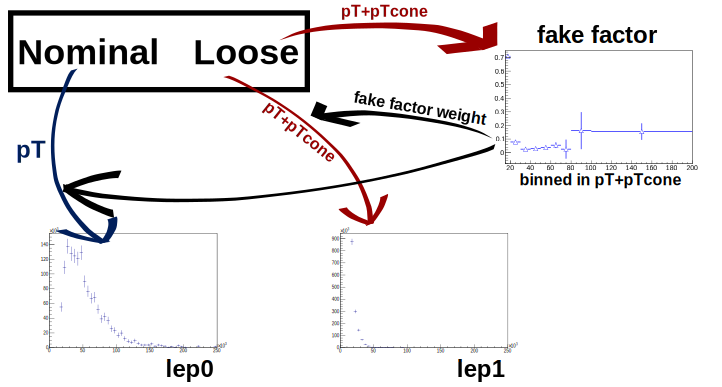
\includegraphics[width=.95\textwidth]{figs/ssww_13tev/backgrounds/ff/apply_ff}
  \caption{Graphical representation of the fake factor application using $\ptptcone$.  The value of $\ptptcone$ for the loose lepton is used to ``look up'' the fake factor weight which is then applied to the event.  The loose lepton's $\pt$ becomes $\ptptcone$ for the purpose of the fake background estimation.}
  \label{fig:ssww13tev_ff_application}
\end{figure}

Finally, it should be noted that the addition of $\ptcone$ to the loose object may cause the loose leptons in the denominator sample to migrate into higher bins.
This results in an overall decrease in the number of loose objects in the lower $\ptptcone$ bins due to there not being additional leptons at lower $\pt$ to replace them.
Since the fake factor is a ratio of the number of events in a bin, this effect causes the first few bins of the fake factor to increase, as can be seen clearly in Figure~\ref{fig:ssww13tev_ff_muon}.
However, the signal and control regions (and their corresponding $NL$ regions) contain a $\pt > 27\gev$ cut that prevents these migrations from negatively impacting the fake estimation.

%---------------------------------------------------------------------------------------------
%
%---------------------------------------------------------------------------------------------
\subsubsection{Systematic uncertainties}\label{ssww13tev:ff_systematics}
Four sources of systematic uncertainty are considered: the dijet event selection, the prompt background subtraction, the jet flavor composition, and residual dependence on the underlying jet $\pt$ spectrum.
In order to measure the impact of these systematics, new fake factors are computed with each of the systematic variations and the differences from the nominal values are taken as the uncertainty.
\begin{enumerate}
\item In order to estimate uncertainties due to the dijet selection, the cut on $M_{\textrm{T}}+\met$ is varied by $\pm5\gev$, $\Delta\phi(l,j)$ by $\pm 0.1$, and the jet $\pt$ cut by $+5\gev$.
\item To estimate the systematic uncertainty on the prompt background subtraction, the MC prediction in a $W$+jets control region is compared to data.  The discrepancy between data and MC is found to be approximately 10\%~\cite{2018.ssww-13tev-atlas-support}.  Therefore, the prompt background used for the subtraction is scaled up and down by $\pm 10\%$.
\item The difference in the jet flavor composition between the dijet events and the events in the $NL$ regions can affect the accuracy of the fake background estimation.  The dijet sample is dominated by light jets, while the $NL$ regions tend to be dominated by heavy flavor from $t\bar{t}$.  To account for this, the fake factor is computed with a $b$-jet veto.
\item To measure any residual dependence on the underlying jet $\pt$ spectrum, the leading jet $\pt$ distribution is reweighted to match the $\pt$ spectrum of truth jets that produce fake leptons in MC simulations.  This results in an increase in the number of nominal and loose leptons at high momentum~\cite{2018.ssww-13tev-atlas-support}.
\end{enumerate}
%An overall uncertainty of 50\% is assigned to the fake background estimation in $\mu^{\pm}\mu^{\pm}$ events, and between 40\% to 90\% for $e^{\pm}e^{\pm}$ and $\mu^{\pm}e^{\pm}$ events, including both statistical and systematic effects.

\begin{figure}[htbp]
  \centering
  \includegraphics[width=.6\textwidth]{figs/ssww_13tev/backgrounds/ff/muon_ff_sys}
  \caption{Systematic variations in the fake factor as a function of muon $\ptptcone$.  The individual fake factors obtained for each systematic variation are displayed with their statistical uncertainties.}
  \label{fig:ssww13tev_ff_muon_sys}
\end{figure}

\begin{figure}[htbp]
  \centering
  \includegraphics[width=.6\textwidth]{figs/ssww_13tev/backgrounds/ff/elec_central_ff_sys}\\
  \includegraphics[width=.6\textwidth]{figs/ssww_13tev/backgrounds/ff/elec_forward_ff_sys}
  \caption{Systematic variations in the fake factor as a function of electron $\ptptcone$ in the central ($|\eta|<1.37$, top) and forward ($|\eta| > 1.37$, bottom) regions of the detector.  The individual fake factors obtained for each systematic variation are displayed with their statistical uncertainties.}
  \label{fig:ssww13tev_ff_elec_sys}
\end{figure}

\begin{table}[hbtp]
  \begin{subtable}{\linewidth}
  \centering
  \resizebox{1.0\textwidth}{!}{
  \begin{tabular}{l|cccccccc}
    fake-factor & $\pt$  [15, 20]      &  $\pt$[20, 27]       &    $\pt$[27, 35]     &    $\pt$[35, 45]     &    $\pt$[45, 55]     &    $\pt$[55, 65]     &    $\pt$[65, 75]     &    $\pt$[75, 200]    \\ \hline\hline
    nominal     & 0.649 $\pm$ 0.007  & 0.083 $\pm$ 0.002 & 0.024 $\pm$ 0.002  & 0.021 $\pm$ 0.003   & 0.044 $\pm$ 0.007   & 0.067 $\pm$ 0.018  & 0.160 $\pm$ 0.055   & 0.481 $\pm$ 0.088 \\ \hline
    \multirow{2}{*}{MT+MET}   & 0.649 $\pm$ 0.007  & 0.082 $\pm$ 0.002   & 0.082 $\pm$ 0.002    & 0.020 $\pm$ 0.003    & 0.045 $\pm$ 0.007 & 0.068 $\pm$ 0.018 & 0.207 $\pm$ 0.062 & 0.523 $\pm$ 0.086 \\
    & 0.648 $\pm$ 0.007 & 0.083 $\pm$ 0.003 & 0.024 $\pm$ 0.002 & 0.022 $\pm$ 0.004 & 0.044 $\pm$ 0.007 & 0.054 $\pm$ 0.020 & 0.207 $\pm$ 0.060 & 0.389 $\pm$ 0.081 \\ \hline
    \multirow{2}{*}{$\Delta\phi(\ell,j)$}    & 0.645 $\pm$ 0.008 & 0.083 $\pm$ 0.003 & 0.024 $\pm$ 0.002 & 0.021 $\pm$ 0.004 & 0.045 $\pm$ 0.008 & 0.064 $\pm$ 0.021 & 0.064 $\pm$ 0.058 & 0.438 $\pm$ 0.092 \\
      & 0.646 $\pm$ 0.006 & 0.083 $\pm$ 0.002 & 0.024 $\pm$ 0.002 & 0.020 $\pm$ 0.003 & 0.043 $\pm$ 0.006 & 0.076 $\pm$ 0.017 & 0.174 $\pm$ 0.050 & 0.448 $\pm$ 0.078 \\ \hline
    Jet $\pt$        & 0.650 $\pm$ 0.007 & 0.083 $\pm$ 0.002 & 0.024 $\pm$ 0.002 & 0.021 $\pm$ 0.003 & 0.045 $\pm$ 0.007 & 0.069 $\pm$ 0.018 & 0.159 $\pm$ 0.018 & 0.481 $\pm$ 0.088 \\ \hline 
    $N_{\textrm{b-jet}} = 0$      & 0.724 $\pm$ 0.003 & 0.094 $\pm$ 0.001 & 0.035 $\pm$ 0.001 & 0.025 $\pm$ 0.002 & 0.022 $\pm$ 0.004 & 0.060 $\pm$ 0.015 & 0.026 $\pm$ 0.053 & 0.044 $\pm$ 0.134 \\ \hline 
    \multirow{2}{*}{Bkg. subtraction}   & 0.648 $\pm$ 0.007 & 0.083 $\pm$ 0.002 & 0.024 $\pm$ 0.002 & 0.019 $\pm$ 0.003 & 0.037 $\pm$ 0.007 & 0.044 $\pm$ 0.019 & 0.096 $\pm$ 0.062 & 0.370 $\pm$ 0.082 \\
    & 0.649 $\pm$ 0.007 & 0.083 $\pm$ 0.002 & 0.025 $\pm$ 0.002 & 0.022 $\pm$ 0.003 & 0.050 $\pm$ 0.007 & 0.090 $\pm$ 0.017 & 0.224 $\pm$ 0.052 & 0.591 $\pm$ 0.099 \\ \hline 
   Jet $\pt$ Reweight & 0.539 $\pm$ 0.077 & 0.093 $\pm$ 0.007 & 0.025 $\pm$ 0.004 & 0.043 $\pm$ 0.019 & 0.063 $\pm$ 0.014 & 0.085 $\pm$ 0.025 & 0.141 $\pm$ 0.110 & 1.962 $\pm$ 0.492 \\ 
    \hline
  \end{tabular}
  }
  \caption{Fake-factor values for muons.}
  \end{subtable}

  \vspace{10mm}

  \begin{subtable}{\linewidth}
  \centering
  \resizebox{1.0\textwidth}{!}{
  \begin{tabular}{l|cccccccc}
    fake-factor   &  $\pt$[20, 27]       &    $\pt$[27, 35]     &    $\pt$[35, 45]     &    $\pt$[45, 55]     &    $\pt$[55, 65]     &    $\pt$[65, 75]     &    $\pt$[75, 200]    \\ \hline\hline
    nominal     & 0.491 $\pm$ 0.031 & 0.140 $\pm$ 0.020 & 0.111 $\pm$ 0.023 & 0.256 $\pm$ 0.049 & 0.546 $\pm$ 0.091 & 0.460 $\pm$ 0.140 & 0.939 $\pm$ 0.125 \\ \hline
    \multirow{2}{*}{MT+MET}   & 0.493 $\pm$ 0.030 & 0.138 $\pm$ 0.019 & 0.115 $\pm$ 0.022 & 0.261 $\pm$ 0.045 & 0.559 $\pm$ 0.084 & 0.656 $\pm$ 0.091 & 0.802 $\pm$ 0.016 \\
                              & 0.488 $\pm$ 0.032 & 0.137 $\pm$ 0.020 & 0.110 $\pm$ 0.025 & 0.283 $\pm$ 0.053 & 0.503 $\pm$ 0.097 & 0.351 $\pm$ 0.149 & 1.117 $\pm$ 0.255 \\ \hline
    \multirow{2}{*}{$\Delta\phi(\ell,j)$}  & 0.489 $\pm$ 0.035 & 0.134 $\pm$ 0.021 & 0.105 $\pm$ 0.025 & 0.224 $\pm$ 0.048 & 0.593 $\pm$ 0.093 & 0.356 $\pm$ 0.144 & 0.928 $\pm$ 0.177 \\ 
     & 0.506 $\pm$ 0.029 & 0.140 $\pm$ 0.018 & 0.111 $\pm$ 0.022 & 0.260 $\pm$ 0.046 & 0.545 $\pm$ 0.084 & 0.546 $\pm$ 0.120 & 0.882 $\pm$ 0.103  \\  \hline
    Jet $\pt$    & 0.493 $\pm$ 0.032 & 0.146 $\pm$ 0.021 & 0.115 $\pm$ 0.024 & 0.259 $\pm$ 0.049 & 0.550 $\pm$ 0.091 & 0.460 $\pm$ 0.140 & 0.939 $\pm$ 0.125 \\ \hline 
    $N_{\textrm{b-jet}} = 0$      & 0.387 $\pm$ 0.009 & 0.130 $\pm$ 0.008 & 0.321 $\pm$ 0.012 & 0.473 $\pm$ 0.015 & 0.716 $\pm$ 0.180 & 0.716 $\pm$ 0.180 & 0.716 $\pm$ 0.180 \\ \hline 
    \multirow{2}{*}{Bkg. subtraction}   & 0.488 $\pm$ 0.031 & 0.138 $\pm$ 0.020 & 0.106 $\pm$ 0.023& 0.248 $\pm$ 0.049 & 0.529 $\pm$ 0.092 & 0.434 $\pm$ 0.143 & 0.888 $\pm$ 0.115 \\ 
      & 0.493 $\pm$ 0.031 & 0.142 $\pm$ 0.020 & 0.115 $\pm$ 0.023 & 0.264 $\pm$ 0.049 & 0.563 $\pm$ 0.090 & 0.485 $\pm$ 0.136 & 0.989 $\pm$ 0.132 \\  \hline
    Jet $\pt$ Reweight     & 0.445 $\pm$ 0.055 & 0.137 $\pm$ 0.037 & 0.065 $\pm$ 0.023 & 0.115 $\pm$ 0.033 & 0.603 $\pm$ 0.047 & 0.104 $\pm$ 0.105 & 0.299 $\pm$ 0.260 \\  
    \hline
  \end{tabular}}
  \caption{Fake-factor values for central electrons ($|\eta| < 1.37$).}
  \end{subtable}

  \vspace{10mm}

  \begin{subtable}{\linewidth}
  \centering
  \resizebox{1.0\textwidth}{!}{
  \begin{tabular}{l|cccccccc}
    fake-factor   &  $\pt$[20, 27]       &    $\pt$[27, 35]     &    $\pt$[35, 45]     &    $\pt$[45, 55]     &    $\pt$[55, 65]     &    $\pt$[65, 75]     &    $\pt$[75, 200]    \\ \hline \hline
    nominal     & 0.487 $\pm$ 0.046 & 0.148 $\pm$ 0.031  & 0.253 $\pm$ 0.046  & 0.412 $\pm$ 0.071  & 0.556 $\pm$ 0.117 & 0.691 $\pm$ 0.117 & 1.340 $\pm$ 0.340 \\ \hline   
 \multirow{2}{*}{MT+MET}   & 0.483 $\pm$ 0.045 & 0.152 $\pm$ 0.031 & 0.241 $\pm$ 0.043 & 0.443 $\pm$ 0.070 & 0.565 $\pm$ 0.106 & 0.668 $\pm$ 0.117 & 1.075 $\pm$ 0.189 \\ 
    & 0.495 $\pm$ 0.047 & 0.156 $\pm$ 0.033 & 0.271 $\pm$ 0.052 & 0.364 $\pm$ 0.074 & 0.664 $\pm$ 0.107 & 0.749 $\pm$ 0.056 & 0.885 $\pm$ 0.084 \\ \hline
    \multirow{2}{*}{$\Delta\phi(\ell,j)$}    & 0.471 $\pm$ 0.051 & 0.158 $\pm$ 0.035 & 0.247 $\pm$ 0.051 & 0.474 $\pm$ 0.085 & 0.283 $\pm$ 0.107 & 0.546 $\pm$ 0.149 & 1.189 $\pm$ 0.266 \\ 
      & 0.478 $\pm$ 0.042 & 0.170 $\pm$ 0.031 & 0.274 $\pm$ 0.046 & 0.389 $\pm$ 0.066 & 0.645 $\pm$ 0.104 & 0.757 $\pm$ 0.102 & 1.319 $\pm$ 0.326 \\ \hline
    Jet $\pt$   & 0.523 $\pm$ 0.048 & 0.149 $\pm$ 0.033 & 0.235 $\pm$ 0.045 & 0.429 $\pm$ 0.073 & 0.555 $\pm$ 0.117 & 0.691 $\pm$ 0.117 & 1.340 $\pm$ 0.340 \\ \hline
    $N_{\textrm{b-jet}} = 0$       & 0.525 $\pm$ 0.011 & 0.234 $\pm$ 0.013 & 0.644 $\pm$ 0.016 & 0.710 $\pm$ 0.014 & 0.274 $\pm$ 0.316 & 0.274 $\pm$ 0.316 & 0.274 $\pm$ 0.316 \\ \hline 
    \multirow{2}{*}{Bkg. subtraction}   & 0.484 $\pm$ 0.046 & 0.146 $\pm$ 0.031 & 0.248 $\pm$ 0.046 & 0.406 $\pm$ 0.071 & 0.545 $\pm$ 0.118 & 0.676 $\pm$ 0.118 & 1.317 $\pm$ 0.337 \\
    & 0.489 $\pm$ 0.046 & 0.151 $\pm$ 0.031 & 0.257 $\pm$ 0.046& 0.419 $\pm$ 0.071 & 0.568 $\pm$ 0.117 & 0.705 $\pm$ 0.115 & 1.363 $\pm$ 0.342 \\    \hline  
    Jet $\pt$ Reweight  & 0.328 $\pm$ 0.068 & 0.124 $\pm$ 0.048 & 0.297 $\pm$ 0.100 & 0.234 $\pm$ 0.061 & 0.680 $\pm$ 0.092 & 0.452 $\pm$ 0.138 & 2.385 $\pm$ 1.729 \\
 \hline
  \end{tabular}}
  \caption{Fake-factor values for forward electrons ($1.37 < |\eta|$).}
  \end{subtable}

  \caption{Values of the fake-factor in each $\pt$ bin and for each individual systematic source.}
  \label{tab:ssww13tev_ff}
\end{table}


%---------------------------------------------------------------------------------------------
%
%---------------------------------------------------------------------------------------------
\subsubsection{Results of the fake factor}\label{ssww13tev:ff_results}
The fake background contribution in the signal region is estimated by applying the fake factors to the equivalent $NL$ region using Equation~\ref{eq:ssww13tev_ff_bkg}, where the fake factor used corresponds to the flavor of the loose lepton in the event.
As usual, the prompt background is subtracted from the $NL$ events using MC simulation.
Charge misidentification is handled using the same method as in Section~\ref{ssww13tev:charge_misid}, with an additional set of charge flip rates calculated for loose leptons.
The fake background yields in the signal region are listed in Table~\ref{tab:ssww13tev_ff_signal_region}.
An overall uncertainty of 50\% is assigned to the fake background estimation in $\mu^{\pm}\mu^{\pm}$ events, and between 40\% to 90\% for $e^{\pm}e^{\pm}$ and $\mu^{\pm}e^{\pm}$ events, including both statistical and systematic effects.

\begin{table}[hbtp]
\centering
  \resizebox{\textwidth}{!}{
  \begin{tabular}{ l | r| r  r  r  r |r  r  r  r }
  & estimated yield & $f_e$ stat.\ up & $f_e$ stat.\ dn & $f_e$ syst.\ up & $f_e$ syst.\ dn & $f_\mu$ stat.\ up & $f_\mu$ stat.\ dn & $f_\mu$ syst.\ up & $f_\mu$ syst.\ dn\\
\hline\hline
$\ee$ & $11.42\pm 3.13$ & $1.69$ & $-1.69$ & $1.67$ & $-5.56$ & --- & --- & --- & ---\\
%\hline
$\mm$ & $4.82\pm 0.77$ & ---  & ---  & ---  & ---  & $0.65$ & $-0.65$ & $3.64$ & $-0.61$\\
%\hline
$\me$ & $37.08\pm 5.16$ & $4.90$ & $-4.90$ & $5.59$ & $-14.34$ & $1.39$ & $-1.39$ & $16.10$ & $-1.98$\\
\hline
\end{tabular}
}
\caption{Estimated yields for the fake lepton background. The estimated yield is shown in the first column together with the statistical uncertainty followed by the systematic uncertainties from variations of the the fake factors within their statistical (stat.) and systematic (syst.) uncertainties. The labels $f_e$ and $f_\mu$ indicate the fake factors for electrons and muons, respectively.}
  \label{tab:ssww13tev_ff_signal_region}
\end{table}

\subsubsection{Validation of the fake factor}\label{ssww13tev:ff_vr}
The accuracy of the fake factor method is tested in several validation regions, the most sensitive of which is the same-sign top fakes VR (SS top VR), defined in Table~\ref{tab:ssww13tev_topfakes_vr_def}.
This region inverts the signal region's $b$-jet veto to accept events with exactly one $b$-jet.
Due to this requirement, the dominant source of events comes from the $t\bar{t}$ process where a $b$-jet fakes an isolated lepton.
The distribution of the subleading lepton $\pt$ in this VR is shown in Figure~\ref{fig:ssww13tev_ff_fakes_vr} for all lepton flavor combinations.
There is good agreement between the data and the prediction, even when only taking into account the statistical uncertainty and not the large systematic uncertainties assigned to the fake estimation.
%The subleading lepton is most likely to be the fake.

\begin{table}[htbp]
  \centering
  \begin{tabular}{c}
    Same-sign inclusive VR \\
    \hline\hline
    Exactly 2 same-sign signal leptons\\
    $\pt > 27\gev$ for both leptons \\
    $m_{ll} > 20\gev$\\
    $|m_{ee} - m_Z| > 15\gev$ ($\ee$-channel only) \\
    $N_{b\textrm{-jet}} = 1$\\
    $N_{\textrm{jet}} \ge 2$ \\
    Leading jet $\pt > 65\gev$ \\
    Subleading jet $\pt > 35\gev$ \\
    \hline
  \end{tabular}
  \caption{Selection criteria for the same-sign top fakes validation region.}
  \label{tab:ssww13tev_topfakes_vr_def}
\end{table}

\begin{figure}
  \centering
  \includegraphics[width=.48\textwidth]{figs/ssww_13tev/backgrounds/ff/fakes_vr/mm-CutCRTopFakesSSZVeto-l1_pt-lin}
  \includegraphics[width=.48\textwidth]{figs/ssww_13tev/backgrounds/ff/fakes_vr/ee-CutCRTopFakesSSZVeto-l1_pt-lin}\\
  \includegraphics[width=.48\textwidth]{figs/ssww_13tev/backgrounds/ff/fakes_vr/emme-CutCRTopFakesSSZVeto-l1_pt-lin}
  \includegraphics[width=.48\textwidth]{figs/ssww_13tev/backgrounds/ff/fakes_vr/ll-CutCRTopFakesSSZVeto-l1_pt-lin}
  \caption{Distributions of the subleading lepton $\pt$ in the same-sign top fakes VR for  $\mm$ events (top right), $\ee$ events (top left), $\me$ events (bottom left), and all events combined (bottom right).  All errors are statistical only.}
  \label{fig:ssww13tev_ff_fakes_vr}
\end{figure} 


\subsection{Reduction of $WZ$ background using custom overlap removal}\label{ssww13tev:custom_or}
The dominant source of prompt background in this analysis comes from $WZ$ events where both bosons decay leptonically.
Traditionally, the background is dealt with by imposing a veto on any event with a third lepton passing some loose identification criteria (the so-called \emph{trilepton veto}).
In the case of this analysis, if one or more leptons (in addition to the two signal leptons) passed the preselection criteria, the event would be rejected.
However, $WZ$ events can still enter the signal region if one of the leptons fails the veto selection or falls outside of the detector's acceptance.

In order to understand the sources of $WZ$ events that are not removed by the trilepton veto, a study was performed on truth-level leptons\footnote{Truth particles are the particles produced directly by the MC generator before being passed through the full detector simulation, at which point they are considered \emph{reconstruction-level} (or \emph{reco-level}) particles.} on \ssww and $WZ$ MC samples.
Events with three truth leptons were selected, and each was matched to its reconstruction-level partner by finding the closest $\deltar(\textrm{truth},\textrm{reco})$ and $\Delta p_{\textrm{T},\textrm{truth},\textrm{reco}}$ match.
For events surviving the trilepton veto, the two signal leptons were removed, and the remaining leptons represent real leptons that failed to be selected for the veto.
Between 40-50\% of these leptons fell outside of the eta acceptance of the analysis (see Figure~\ref{fig:ssww13tev_wzveto_truthlepeta}) and were unrecoverable.
The second largest source of leptons failing the preselection was the OR, defined in Section~\ref{ssww13tev:overlap_removal}.
The standard OF procedure appeared to be too aggressive in removing leptons in favor of jets, causing many three lepton events to ``lose'' their third lepton and pass the trilepton veto.
Therefore a \emph{Custom OR} was investigated which would replace the standard OR in the preselection and allow for better $WZ$ rejection by removing fewer third leptons.

\TODO{Mention how the extra leptons in the \ssww are background leptons since there are only 2 from the main decay}

\begin{figure}[htbp]
  \centering
  \includegraphics[width=.48\textwidth]{figs/ssww_13tev/custom_or/ExtraMuonEta_counted}
  \includegraphics[width=.48\textwidth]{figs/ssww_13tev/custom_or/ExtraElecEta_counted}
  \caption{Pseudorapidity ($\eta$) distributions of truth muons (top) and electrons (bottom) for Sherpa \ssww and $WZ$ MC samples.  The blue vertical lines represent the allowed $\eta$ range for each lepton flavor.  The numbers correspond to the number of raw MC events that fall within and outside of the allowed $\eta$ range for each MC sample.}
  \label{fig:ssww13tev_wzveto_truthlepeta}
\end{figure}

In order to construct a ``custom'' OR, a new quantity is defined between a lepton ($l$) and a nearby jet ($j$)
\begin{equation}
  \ptratio(l,j) = \frac{{\pt}_l}{{\pt}_j}%\pt(l)/\pt(j)
  \label{eq:ssww13tev_ptratio}
\end{equation}
which, along with $\deltar(l,j)$, will allow for more third leptons to pass the preselection.
The idea behind including $\ptratio$ is to be able to preferentially remove background leptons originating from jets (i.e. those that carry a low percentage of the total jet momentum) instead of removing \emph{any} lepton near to jet.
The distributions of $\ptratio$ and the associated efficiency curves for muons and electrons can be found in Figures~\ref{fig:ssww13tev_ptratio_muon} and \ref{fig:ssww13tev_ptratio_elec}, respectively, and the distributions for $\deltar(\mu,j)$ for muons can be found in Figure~\ref{fig:ssww13tev_drlj_muon}.
Since all electrons have an associated jet in the calorimeters, the $\deltar(e,j)$ variable is not a good quantity to use for this custom OR.

\begin{figure}[htbp]
  \centering
  \includegraphics[width=.48\textwidth]{figs/ssww_13tev/custom_or/VetoMuonPtRatiolj}
  \includegraphics[width=.48\textwidth]{figs/ssww_13tev/custom_or/ROC_VetoMuonPtRatiolj}
  \caption{Distributions of $\ptratio(\mu,j)$ for EWK and QCD \ssww signal (black) and $WZ$ background (teal) for truth-matched third muons in events that pass the trilepton veto.  Both distributions are normalized to unit area.  The associated efficiency curves are on the right where efficiency is defined as the percentage of total events that would pass a cut on $\ptratio(\mu,j)$ at a given value on the $x$-axis.}
  \label{fig:ssww13tev_ptratio_muon}
\end{figure}

\begin{figure}[htbp]
  \centering      
  \includegraphics[width=.48\textwidth]{figs/ssww_13tev/custom_or/veto_muon_VetoDRlj}
  \includegraphics[width=.48\textwidth]{figs/ssww_13tev/custom_or/ROC_veto_muon_VetoDRlj}\\
  \caption{Distributions of $\deltar(\mu,j)$ for EWK and QCD \ssww signal (black) and $WZ$ background (teal) for truth-matched third muons in events that pass the trilepton veto.  Both distributions are normalized to unit area.  The associated efficiency curves are on the right where efficiency is defined as the percentage of total events that would pass a cut on $\deltar(\mu,j)$ at a given value on the $x$-axis.}
  \label{fig:ssww13tev_drlj_muon}
\end{figure}

\begin{figure}[htbp]
  \centering
  \includegraphics[width=.48\textwidth]{figs/ssww_13tev/custom_or/VetoElecPtRatiolj}
  \includegraphics[width=.48\textwidth]{figs/ssww_13tev/custom_or/ROC_VetoElecPtRatiolj}
  \caption{Distributions of $\ptratio(e,j)$ for EWK and QCD \ssww signal (black) and $WZ$ background (teal) for truth-matched third electrons in events that pass the trilepton veto.  Both distributions are normalized to unit area.  The associated efficiency curves are on the right where efficiency is defined as the percentage of total events that would pass a cut on $\ptratio(e,j)$ at a given value on the $x$-axis.}
  \label{fig:ssww13tev_ptratio_elec}
\end{figure}

A workingpoint for the Custom OR was chosen by requiring 90\% signal retention for muons and 90\% background rejection for electrons.
The cut on electrons was allowed to be much tighter because the number of signal events with a third electron is considerably smaller than for muons.
It should be re-emphasized the signal events that are present in Figures~\ref{fig:ssww13tev_ptratio_muon}-\ref{fig:ssww13tev_ptratio_elec} do not represent the full set of signal events, but only those with a real third lepton (which must come from some source other than the signal \ssww process).
For muons, an or of $\ptratio(\mu,j)$ and $\deltar(\mu,j)$ is used to maximize the third lepton acceptance due to correlations between the quantities, as shown in Figure~\ref{fig:ssww13tev_customor_muon_2d}; for electrons, only a cut on $\ptratio(e,j)$ is used.
The Custom OR workingpoint is outlined in Table~\ref{tab:custom_or_definition}.

\begin{table}[htbp]
  \centering
  \begin{tabular}{l | c}
    \multicolumn{2}{c}{Custom OR Definition} \\
    \hline\hline
    Muons     & $\ptratio(\mu,j) > 0.40$ or $\deltar(\mu,j) > 0.15$\\
    Electrons & $\ptratio(e,j) > 0.18$ \\
    \hline
  \end{tabular}
  \caption{Custom OR definition.  Leptons must pass this selection in order to be counted for the trilepton veto.}
  \label{tab:custom_or_definition}
\end{table}

\begin{figure}[htbp]
  \centering
  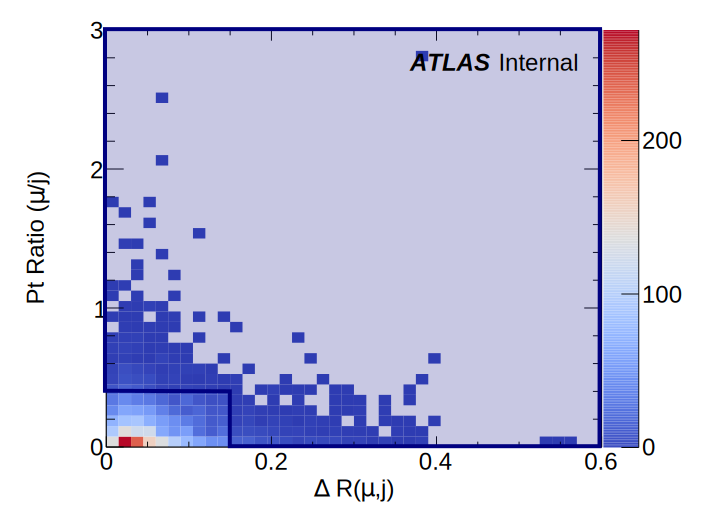
\includegraphics[width=.48\textwidth]{figs/ssww_13tev/custom_or/sig_Muon_DR_PtRatio_edited}
  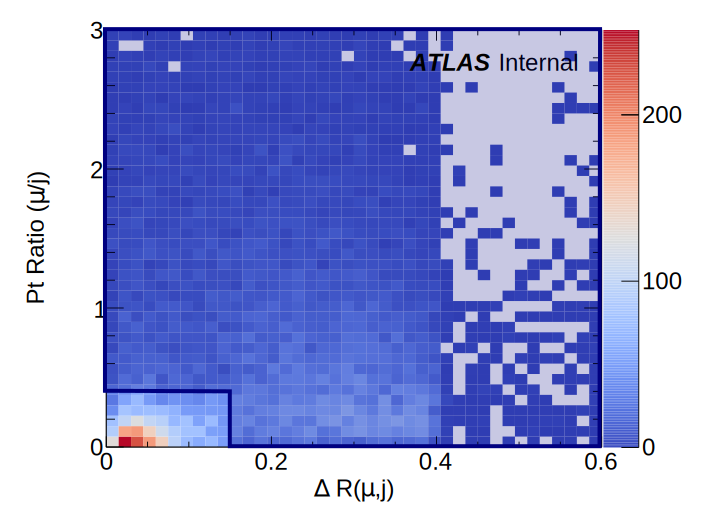
\includegraphics[width=.48\textwidth]{figs/ssww_13tev/custom_or/bkg_Muon_DR_PtRatio_edited}
  \caption{Two-dimensional plots of $\ptratio(\mu,j)$ vs $\deltar(\mu,j)$ for truth-matched third muons in events that pass the trilepton veto for EWK and QCD \ssww signal (left) and $WZ$ background (right).  The blue overlay indicates the area in which the third leptons will pass the custom OR and result in the event failing the trilepton veto.}
  \label{fig:ssww13tev_customor_muon_2d}
\end{figure}

Tests of the performance of the Custom OR yield promising results, with approximately 20\% reduction in $WZ$ background compared to less than 2\% signal loss in the signal region.
Unfortunately, due to differences between the primary analysis framework and the one used for testing, in practice the gains in $WZ$ rejection are not nearly as substantial, and ultimately the Custom OR is not included in the final analysis.
However, it is still a potentially useful tool for improving background rejection via lepton number vetoes in analyses with overly aggressive OR procedures.



\section{Cross section measurement}\label{ssww13tev:xsec}
% for now, I'm only goint to talk about the measured (observed) fit and cross section stuff, since ultimately that's the result of interest
% it's the real important bit, and also easier to understand since the statistical modelling with the Asimov data is a bit confusing...

The \ssww EWK cross section is extracted from the signal region using a maximum-likelihood fit applied simultaneously to four $m_{jj}$ bins in the signal region as well as to the low-$m_{jj}$ and $WZ$ control regions.
For the fit and cross section extraction, the signal region is defined as in Table~\ref{tab:ssww13tev_event_selection} with the dijet invariant mass requirement raised to $m_{jj} > 500\gev$.
The low-$m_{jj}$ region is defined to mirror the signal region exactly with the dijet invariant mass inverted to $200 < m_{jj} < 500\gev$, and the $WZ$ control region is as defined previously in Section~\ref{ssww13tev:wz}.

The signal and low-$m_{jj}$ regions are split into six channels based on the flavor and charge of the dilepton pair: $\mmp$, $\mmm$, $\mep$, $\mem$, $\eep$, and $\eem$.
This split by charge increases the sensitivity of the measurement due to the $W^{+}/W^{-}$ charge asymmetry favoring the production of $W^{+}$ bosons~\cite{2010.w-charge-asymmetry}.
Since the signal events contain two $W$ bosons, the signal strength compared to charge-symmetric backgrounds is much greater in the $++$ channels than for both charges combined.
The $WZ$ control region is included in the fit as a single bin ($l^{\pm}l^{\mp}l^{\pm}$).

The maximum likelihood fit and cross section extractions are outlined in Sections~\ref{ssww13tev:xsec_fit_method} and \ref{ssww13tev:xsec_method}, respectively.
The results of the cross section measurement and of the analysis as a whole are presented in Section~\ref{ssww13tev:results}.

\subsection{Maximum likelihood fit}\label{ssww13tev:xsec_fit_method}
%\TODO{This section is very similar to what is written in the support note... May need to put some work into flushing it out so it's not so close to copy-paste}
The number of predicted signal events in each channel $c$ and $m_{jj}$ bin $b$ can be calculated from the SM predicted total production cross section $\sigma^{\textrm{tot}}_{\textrm{theo}}$ scaled by the total integrated luminosity $\mathcal{L}$, the signal acceptance $\mathcal{A}$, and the efficiency corrections $\mathcal{C}(\theta)$:
\begin{equation}
  N_{cb}^{\textrm{sig}}(\theta) = \sigma^{\textrm{tot}}_{\textrm{theo}}\mathcal{A}_b\mathcal{C}_{b}(\theta)\mathcal{L}\,.
  \label{eq:ssww13tev_xsec_nsig}
\end{equation}
Here, $\theta$ represents the set of nuisance parameters that parameterize the effects of each systematic uncertainty on the signal and background expectations.
The acceptance and efficiency corrections will be covered in more detail in Section~\ref{ssww13tev:xsec_fid_vol}.
A signal strength parameter $\mu$ is defined as the ratio of the measured cross section to the SM predicted cross section.
%it seems like $\mu$ is the main thing we're extracting from the fit, and we calculate the cross section by measuring $\mu$ and solving for $\sigma_obs$, maybe put some words about this in
The expected number of events in a given channel and bin can then be expressed as the sum of the estimated background ($N_{cb}^{\textrm{bkg}}(\theta)$) and the number of predicted signal events scaled by $\mu$:
\begin{equation}
  \begin{aligned}
    N_{cb}^{\textrm{exp}}(\theta) &= \mu N_{cb}^{\textrm{sig}}(\theta) + N_{cb}^{\textrm{bkg}}(\theta) \\
                              &= \mu \sigma^{\textrm{tot}}_{\textrm{theo}}\mathcal{A}_b\mathcal{C}_{b}(\theta)\mathcal{L} + N_{cb}^{\textrm{bkg}}(\theta)\,.
  \end{aligned}
  \label{eq:ssww13tev_xsec_nexp}
\end{equation}

The nuisance parameters are constrained by Gaussian probability distribution functions, and the normalization of the $WZ$ background mentioned in Section~\ref{ssww13tev:wz} is included in the fit as a free parameter.
The expected yields for signal and background processes are adjusted by the set of nuisance parameters within the constraints of the systematic uncertainties.
The yields after the fit correspond to the value that best matches the observed data.

The number of events per channel and bin after the fit can be written as a sum of the predicted event yields for each sample $s$:
\begin{equation}
  \nu_{cb}(\phi,\theta,\gamma_{cb}) = \gamma_{cb}\sum\limits_{s}\big[\eta_{cs}(\theta)\phi_{cs}(\theta)\lambda\big] h_{cbs}(\theta)\,.
  \label{eq:ssww13tev_xsec_nexp_fit}
\end{equation}
In this equation, the fitted number of events in a given channel and bin is obtained by weighting the histogram of predicted yields $h_{cbs}$ by the product of a given luminosity $\lambda$ and any normalization factors $\phi_{cs}$ that may be given for each channel and sample.
The input histogram and the normalization factors may depend on the nuisance parameters $\theta$ taking into account sources of systematic uncertainty.
Uncertainties on the normalization factors $\eta_{cs}(\theta)$ are also included.
Finally, bin-by-bin scale factors $\gamma_{cb}$ are included to parameterize the statistical uncertainties of the MC predictions.

The binned likelihood function is given by a product of Gaussian functions for the luminosity and for the background uncertainties and a product of Poisson functions for the number of observed events in each bin and channel:
\begin{equation}
  L(\mu|\theta) = \mathcal{G}(\mathcal{L}|\theta_{\mathcal{L}},\sigma_{\mathcal{L}})\cdot \prod\limits_{c}\prod\limits_{b}\mathcal{P}(N_{\textrm{cb}}^{\textrm{meas.}}|\nu_{cb}(\mu))\prod\limits_{p}\mathcal{G}(\theta_{p}^{0}|\theta_{p})\,,
\end{equation}
where $\mathcal{G}$ and $\mathcal{P}$ are the Gaussian and Poisson functions, respectively.
As before, $\mathcal{L}$ represents the integrated luminosity with uncertainty $\sigma_{\mathcal{L}}$ and associated nuisance parameter $\theta_{\mathcal{L}}$.
The number of measured events in a given bin and channel is represented by $N_{cb}^{\textrm{meas.}}$, and $\nu_{cb}(\mu)$ is the predicted number of events defined in Equation~\ref{eq:ssww13tev_xsec_nexp_fit} expressed as a function of the signal strength $\mu$.
Finally, the set of nuisance parameters $\theta$ and any auxiliary measurements used to constrain them ($\theta^0$) are multiplied for each parameter $p$.

The profile likelihood ratio is defined as
\begin{equation}
  q_{\mu} = -2\ln\frac{L(\mu,\hat{\hat{\theta}}_{\mu})}{L(\hat{\mu},\hat{\theta})}\,,
  \label{dq:ssww13tev_xsec_test_statistic}
\end{equation}
where $\hat{\mu}$ and $\hat{\theta}$ are the unconditional maximum likelihood estimates, and $\hat{\hat{\theta}}$ is the conditional maximum likelihood estimate for a given value of $\mu$.
%basically the idea here is that the unconditional maximum is just the best value of \theta and \mu.  the conditional maximum is the best value of \theta GIVEN a particular \mu (i.e. the best value of \theta is conditional upon the choice of \mu)
%Since $q_{\mu}$ is asymptotically $\chi^2$ distributed according to Wilks' theorem~\cite{}
The fitted signal strength $\hat{\mu}$ is obtained by maximizing the likelihood function with respect to all parameters.
The compatibility of the observed data with the background-only hypothesis can then be calculated by setting $\mu=0$.
Observation of the \ssww EWK process is claimed if the data is found to be inconsistent with the background-only hypothesis by more than $5\sigma$.
%The observed signal strength $\mu_{\textrm{obs}}$ is obtained by using the real data yields in each input bin to the fit; calculating the expected signal strength $\mu_{\textrm{exp}}$ follows the same method but with the data replaced by the predictions from simulation and data-driven estimations.

%\subsection{Results of the fit}\label{ssww13tev:xsec_fit_results}
%To measure the expected significance, 

\subsection{Definition of the fiducial volume}\label{ssww13tev:xsec_fid_vol}
Before extracting the cross section, it is necessary to define the fiducial volume, or the phase space of measurable events.
It is a subset of the total phase space defined by selection requirements designed to mirror those applied in the analysis as closely as possible
The selection criteria for the fiducial volume are listed in Table~\ref{tab:ssww13tev_fiducial_vol}.

\begin{table}[htbp]
  \centering
  \begin{tabular}{l | l}
    \multicolumn{2}{c}{Fiducial region selection} \\
    \hline\hline
    \multirow{5}{*}{Lepton selection} & Two prompt leptons ($e$, $\mu$) \\
    & $\pt > 27\gev$ and $|\eta| < 2.5$ for both leptons \\
    & Both leptons with the same electric charge \\
    & Dilepton invariant mass $m_{ll} > 20\gev$\\
    & Dilepton separation $\deltar (ll) > 0.3$\\
    \hline
    Missing transverse energy & Two neutrino system with $\pt^{\nu\nu} > 30\gev$ \\
    \hline
    \multirow{7}{*}{Jet selection} & At least two jets \\
    & Leading jet $\pt > 65\gev$ \\
    & Subleading jet $\pt > 35\gev$ \\
    & Leading and subleading jet $|\eta| < 4.5$ \\
    & Jet-lepton separation $\deltar (l,j) > 0.3$ \\
    & Dijet invariant mass $m_{jj} > 500\gev$\\
    & Dijet separation $\Delta y_{jj} > 2.0$ \\
    \hline    
  \end{tabular}
  \caption{Definition of the fiducial volume.}
  \label{tab:ssww13tev_fiducial_vol}
\end{table}

The full phase space is generated in MC simulations, providing the total theoretical cross section $\sigmatottheo$
and the total number of signal events $\mathcal{N}_{\textrm{sig}}^{\textrm{tot}}$\footnote{For the purpose of clarity, the number of events at truth level is represented by a script $\mathcal{N}$, and the number of events at reconstruction level uses a regular $N$.}.
After applying the fiducial selection at truth level, the total number of signal events in the fiducial region $\mathcal{N}_{\textrm{sig}}^{\textrm{fid}}$ is obtained.
%, and the fiducial predicted cross section can be written in terms of an acceptance factor $\mathcal{A}$ first introduced in Equation~\ref{eq:ssww13tev_xsec_nsig}:
An acceptance factor $\mathcal{A}$ is used to represent the efficiency of events falling inside the fiducial region at truth level:
\begin{equation}
  \mathcal{A} = \frac{\mathcal{N}_{\textrm{sig}}^{\textrm{fid}}}{\mathcal{N}_{\textrm{sig}}^{\textrm{tot}}}\,.
  \label{eq:ssww13tev_xsec_acceptance}
\end{equation}
A correction factor $\mathcal{C}$ is also necessary to translate from the truth level fiducial volume to the reconstruction level signal region and is defined in terms of the number of reconstruction level MC events in the signal region $N_{\textrm{sig,MC}}^{\textrm{SR}}$:
\begin{equation}
  \mathcal{C} = \frac{N_{\textrm{sig,MC}}^{\textrm{SR}}}{\mathcal{N}_{\textrm{sig}}^{\textrm{fid}}}\,.
  \label{eq:ssww13tev_xsec_efficiency}
\end{equation}
Since the fit is binned in $m_{jj}$, the acceptance and efficiency correction factors must be as well.
Therefore, $\mathcal{A}_i$ and $\mathcal{C}_{ij}$ are written in terms of truth $m_{jj}$ bins $i$ and reconstruction $m_{jj}$ bins $j$.
A graphical representation of these regions and the use of the acceptance and correction factors can be seen in Figure~\ref{fig:ssww13tev_xsec_fiducial_graphic}.

\begin{figure}[htbp]
  \centering
  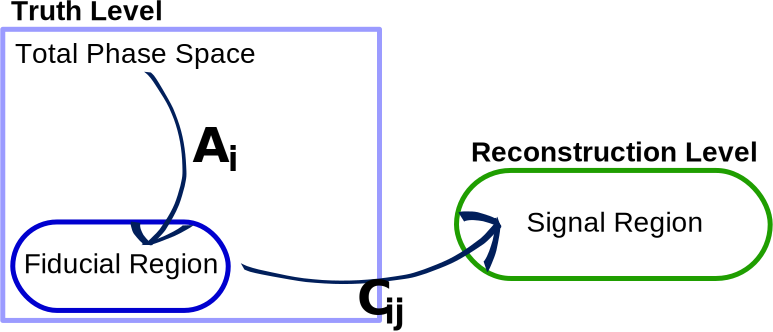
\includegraphics[width=.8\textwidth]{figs/ssww_13tev/xsec/fiducial}
  \caption{Visual representation of the different kinematic regions relevant to the cross section measurement.  The acceptance factor $\mathcal{A}$ converts from the truth level total phase space to the truth level fiducial region, and the efficiency correction $\mathcal{C}$ translates the fiducial region in to the reconstruction level signal region.}
  \label{fig:ssww13tev_xsec_fiducial_graphic}
\end{figure}

\subsection{Cross section extraction}\label{ssww13tev:xsec_method}
The \ssww EWK fiducial cross section is measured using the signal strength parameter $\mu$ that is determined by the maximum likelihood fit.
This parameter is dependent on the nuisance parameters $\theta$ and can be written explicitly in terms of the measured and theoretical cross sections as
\begin{equation}
  \mu(\theta) = \frac{\sigma_{\textrm{meas}}^{\textrm{SR}}}{\sigma_{\textrm{theo}}^{\textrm{SR}}}\,.
  \label{eq:ssww13tev_xsec_mu}
\end{equation}

In the simple case with only one bin, the equation for the total number of expected events in the signal region first introduced in Equation~\ref{eq:ssww13tev_xsec_nexp} can be written as
\begin{equation}
  N_{\textrm{exp}}^{\textrm{SR}}(\theta) = \mu(\theta)\cdot\sigmatottheo\cdot\mathcal{L}\cdot\mathcal{A}\cdot\mathcal{C}(\theta)+N_{\textrm{bkg}}^{\textrm{SR}}(\theta)
  \label{eq:ssww13tev_xsec_nexp_unbinned}
\end{equation}
with the unbinned versions of $\mathcal{A}$ and $\mathcal{C}$ defined in Equations~\ref{eq:ssww13tev_xsec_acceptance} and \ref{eq:ssww13tev_xsec_efficiency}, respectively.

If the measured fiducial cross section is written as
\begin{equation}
  \sigma_{\textrm{meas}}^{\textrm{fid}} = \mu\cdot\mathcal{A}\cdot\sigmatottheo\,,
\end{equation}
then Equation~\ref{eq:ssww13tev_xsec_nexp_unbinned} can be rearranged to read
\begin{equation}
  \sigma_{\textrm{meas}}^{\textrm{fid}} = \frac{N_{\textrm{exp}}^{\textrm{SR}}(\theta)-N_{\textrm{bkg}}^{\textrm{SR}}(\theta)}{\mathcal{L}\cdot\mathcal{C}(\theta)}\,.
  \label{eq:ssww13tev_xsec_fid_meas}
\end{equation}
The measured fiducial cross section can finally be rewritten in terms of $\hat{\mu}$, which is the best estimator of the signal strength as extracted from the fit:
\begin{equation}
  \begin{aligned}
    \sigma_{\textrm{meas}}^{\textrm{fid}} &= \hat{\mu}(\theta)\cdot\sigmatottheo\cdot\mathcal{A}\\
    &= \hat{\mu}(\theta)\cdot\sigma_{\textrm{theo}}^{\textrm{fid}}\,.
  \end{aligned}
  \label{eq:ssww13tev_xsec_fid_meas_mu}
\end{equation}

In practice, however, the cross section is not extracted from a single bin, and Equation~\ref{eq:ssww13tev_xsec_nexp_unbinned} becomes
\begin{equation}
  N_{\textrm{exp}}^{\textrm{SR}}(\theta) = \mu(\theta)\cdot\sigmatottheo\cdot\mathcal{L}\cdot\sum\limits_i\mathcal{A}_i\sum\limits_j\mathcal{C}_{ij}+\sum\limits_j N_{\textrm{bkg},j}^{\textrm{SR}}(\theta)
\end{equation}
for a single channel in truth and reconstruction level $m_{jj}$ bins $i$ and $j$, respectively, where the binned versions of $\mathcal{A}_i$ and $\mathcal{C}_{ij}$ are used.
This equation can be extended to include all the analysis channels by increasing the number of bins $i$ and $j$.
Additionally, it can be shown that Equation~\ref{eq:ssww13tev_xsec_fid_meas_mu} holds for this more complex case as well~\cite{2018.ssww-13tev-atlas-support}, provided care is taken to ensure that all the uncertainties are handled properly.

%\begin{equation}
%  \begin{aligned}
%    N_{\textrm{sig,MC},j} ^{\textrm{SR}}(\theta) &= \sum\limits_i\mathcal{C}_{ij}(\theta)\cdot\mathcal{N}_{\textrm{sig}}^{\textrm{fid}}\\
%    &= \sum\limits_i\mathcal{C}_{ij}(\theta)\big(\mathcal{L}\mathcal{A}_i\sigmatottheo\big)
%  \end{aligned}
%\end{equation}
%then the expected number of signal events in the signal region becomes:
%\begin{equation}
%  N_{\textrm{exp}}^{\textrm{SR}}(\theta) = \mu(\theta)\sum\limits_j N_{\textrm{sig,MC},j}^{\textrm{SR}}(\theta)
%\end{equation}

%\subsection{Results of the cross section measurement}\label{ssww13tev:xsec_results}
%The theoretical fiducial cross section of \ssww EWK production is calculated using \sherpav{2.2.2}.
%The cross section in the total generator phase space is $40.81\pm 0.05\textrm{fb}$, and the fiducial cross section is $2.01\pm 0.02\textrm{fb}$.
%This corresponds to an acceptance factor of $\mathcal{A} = 0.0493\pm 0.0002$.
%Uncertainties on the simulation are estimated using variations of the scale, parton shower, and PDF set.
%The final prediction used in the cross section measurement including uncertainty is:
%\begin{equation}
%  \sigma_{\tt{SHERPA}}^{\textrm{fid}} = 2.01 \pm 0.02(\textrm{stat})~^{+0.29}_{-0.23} (\textrm{scale})~^{+0.16}_{-0.02}(\textrm{parton shower})~^{+0.05}_{-0.03} (\textrm{PDF})~\textrm{fb}
%\end{equation}


\section{Results}\label{ssww13tev:results}
%\TODO{Observed fit results: support note 9.7 p. 138}

After running the full analysis chain, the event yields in the signal region, low-$m_{jj}$ control region, and $WZ$ control region as well as associated nuisance parameters representing the uncertainties are passed to the maximum likelihood fit.
From this fit, the normalization factor for the $WZ$ control region $\mu_{WZ}$ and the signal strength parameter in the signal region $\mu_{\textrm{obs}}$ are determined, and the predicted yields in each input bin have been shifted according to the process detailed in Section~\ref{ssww13tev:xsec_fit_method}.

The $WZ$ normalization factor is measured to be:
\begin{equation}
  \mu_{WZ} = 0.88^{+0.07}_{-0.07}(\textrm{stat})~^{+0.31}_{-0.21}(\textrm{theory})~^{+0.22}_{-0.11}(\textrm{sys})
  \label{eq:ssww13tev_signal_strength_wz}
\end{equation}
and is constrained primarily by the number of data events in the $WZ$ control region.
The observed signal strength of \ssww EWK production, defined in Equation~\ref{eq:ssww13tev_xsec_mu}, is extracted from the fit and measured with respect to the prediction of the \sherpav{2.2.2} MC generator:
\begin{equation}
  \mu_{\textrm{obs}} = 1.45^{+0.25}_{-0.24}(\textrm{stat})~^{+0.06}_{-0.08}(\textrm{theory})~^{+0.27}_{-0.22}(\textrm{sys}) % paper has no theory uncert for some reason
  \label{eq:ssww13tev_signal_strength_sr}
\end{equation}
This corresponds to a rejection of the background-only hypothesis with a significance of $6.9\sigma$.

The observed number of data events are compared to the predicted signal and background yields in the signal region in Table~\ref{tab:ssww13tev_yields_prefit} before applying the fit and in Table~\ref{tab:ssww13tev_yields_postfit} after the fit.
122 candidate events are observed compared to a prediction of 60 signal and 69 background events.

The $m_{jj}$ distributions for data and prediction are shown in Figure~\ref{fig:ssww13tev_results_mjj_sr_postfit} after the fit, and the fitted event yields in the low-$m_{jj}$ and $WZ$ control regions are shown in Figure~\ref{fig:ssww13tev_results_cr_postfit}.
Additional distributions can be found in Appendix~\ref{app:ssww13tev_additional_material}.

\begin{table}[htbp]
  \resizebox{\linewidth}{!}{
  \begin{tabular}{l|l@{$\,\pm\,$}ll@{$\,\pm\,$}ll@{$\,\pm\,$}ll@{$\,\pm\,$}ll@{$\,\pm\,$}ll@{$\,\pm\,$}l|l@{$\,\pm\,$}l}
    & \multicolumn{2}{c}{$\eep$}& \multicolumn{2}{c}{$\eem$}& \multicolumn{2}{c}{$\mep$}& \multicolumn{2}{c}{$\mem$}& \multicolumn{2}{c}{$\mmp$}& \multicolumn{2}{c|}{$\mmm$}& \multicolumn{2}{c}{combined}\\
\hline\hline
$WZ$                    & 1.9 & 0.6 & 1.3 & 0.4 & 14 & 4 & 8.9 & 2.6 & 5.5 & 1.6 & 3.6 & 1.1 & 35 & 10 \\ % before scaling (calculated by hand)
Non-prompt            & 4.1& 2.3   & 2.3& 1.7   & 9& 5   & 6& 4   & 0.57& 0.15   & 0.67& 0.25   & 23& 10 \\
$e/\gamma$ conversions         & 1.74& 0.29   & 1.8& 0.4   & 6.1& 1.6   & 3.7& 0.8   & \multicolumn{2}{c}{---}   & \multicolumn{2}{c|}{---}   & 13.4& 2.5 \\
Other prompt          & 0.17& 0.05   & 0.14& 0.04   & 0.90& 0.19   & 0.60& 0.14   & 0.36& 0.10   & 0.19& 0.05   & 2.4& 0.5 \\
\ssww QCD              & 0.38& 0.13   & 0.16& 0.05   & 3.0& 1.0   & 1.2& 0.4   & 1.8& 0.6   & 0.76& 0.25   & 7.3& 2.5 \\
\hline
Expected background   & 8.2 & 2.4 & 5.7 & 1.8 & 33 & 7 & 21 & 5 & 8.2 & 1.8 & 5.3 & 1.2 & 81 & 14  \\
\hline
\ssww EWK & 3.8 & 0.6 & 1.49 & 0.22 & 16.5 & 2.5 & 6.5 & 1.0 & 9.1 & 1.4 & 3.5 & 0.5 & 41 & 6 \\
\hline
Data& \multicolumn{2}{c}{10}& \multicolumn{2}{c}{4}& \multicolumn{2}{c}{44}& \multicolumn{2}{c}{28}& \multicolumn{2}{c}{25}& \multicolumn{2}{c|}{11}& \multicolumn{2}{c}{122}\\
\hline
\end{tabular}
  }
  \caption{Table of the data and prediction event yields in the signal region before the fit.  Numbers are shown for the six lepton flavor and charge channels and for all channels combined.  Here the $WZ$ background yields are normalized to the data in the $WZ$ control region.  The background estimations from the fake factor are included in the ``Non-prompt'' category, and backgrounds from  $V\gamma$ production and electron charge misidentification are combined in the ``$e/\gamma$ conversions'' category. Finally, $ZZ$, $VVV$, and $t\bar{t}V$ backgrounds are combined in the ``Other prompt'' category.}
  \label{tab:ssww13tev_yields_prefit}
\end{table}

\begin{table}[htbp]
  \resizebox{\linewidth}{!}{
    \begin{tabular}{l|l@{$\,\pm\,$}ll@{$\,\pm\,$}ll@{$\,\pm\,$}ll@{$\,\pm\,$}ll@{$\,\pm\,$}ll@{$\,\pm\,$}l|l@{$\,\pm\,$}l}
    & \multicolumn{2}{c}{$\eep$}& \multicolumn{2}{c}{$\eem$}& \multicolumn{2}{c}{$\mep$}& \multicolumn{2}{c}{$\mem$}& \multicolumn{2}{c}{$\mmp$}& \multicolumn{2}{c|}{$\mmm$}& \multicolumn{2}{c}{combined}\\
    \hline\hline
    $WZ$                    & 1.49& 0.30   & 1.10& 0.26   & 11.7& 1.7   & 8.0& 1.3   & 5.0& 0.6   & 3.5& 0.6   & 31& 4 \\
    Non-prompt            & 2.2& 1.3   & 1.2& 0.7   & 5.7& 2.8   & 4.5& 1.8   & 0.57& 0.06   & 0.65& 0.14   & 15& 6 \\
    $e/\gamma$ conversions           & 1.6& 0.4   & 1.6& 0.5   & 6.3& 1.6   & 4.3& 1.1   & \multicolumn{2}{c}{---} & \multicolumn{2}{c|}{---}   & 13.8& 2.9 \\
    Other prompt          & 0.16& 0.04   & 0.14& 0.04   & 0.90& 0.19   & 0.63& 0.13   & 0.39& 0.09   & 0.22& 0.05   & 2.4& 0.5 \\
    \ssww QCD              & 0.35& 0.13   & 0.15& 0.05   & 2.9& 1.0   & 1.2& 0.4   & 1.8& 0.6   & 0.76& 0.25   & 7.2& 2.4 \\
    \hline
    Expected background   & 5.8& 1.5   & 4.1& 1.1   & 27& 4   & 18.7& 2.6   & 7.7& 0.8   & 5.1& 0.6   & 69& 7 \\
    \hline
    \ssww EWK            & 5.6& 1.0   & 2.2& 0.4   & 24& 5   & 9.4& 1.8   & 13.5& 2.5   & 5.2& 1.0   & 60& 11 \\
    \hline
    Data& \multicolumn{2}{c}{10}& \multicolumn{2}{c}{4}& \multicolumn{2}{c}{44}& \multicolumn{2}{c}{28}& \multicolumn{2}{c}{25}& \multicolumn{2}{c|}{11}& \multicolumn{2}{c}{122}\\
    \hline
    \end{tabular}
  }
  \caption{Table of the data and prediction event yields in the signal region after the fit.  Numbers are shown for the six lepton flavor and charge channels and for all channels combined.  The background estimations from the fake factor are included in the ``Non-prompt'' category, and backgrounds from  $V\gamma$ production and electron charge misidentification are combined in the ``$e/\gamma$ conversions'' category.  Finally, $ZZ$, $VVV$, and $t\bar{t}V$ backgrounds are combined in the ``Other prompt'' category.}
  \label{tab:ssww13tev_yields_postfit}
\end{table}

\begin{figure}[htbp]
  \centering
  \includegraphics[width=.6\textwidth]{figs/ssww_13tev/results/mjj_postfit_all}
  \caption{The dijet invariant mass $m_{jj}$ distributions for data and predicted signal and background in the signal region after the fit.  The shaded band represents the statistical and systematic uncertainties added in quadrature.  Note that the bins have been scaled such that they represent the number of events per $100\gev$ in $m_{jj}$.  The background estimations from the fake factor are included in the ``Non-prompt'' category, and backgrounds from  $V\gamma$ production and electron charge misidentification are combined in the ``$e/\gamma$ conversions'' category.  Finally, $ZZ$, $VVV$, and $t\bar{t}V$ backgrounds are combined in the ``Other prompt'' category.}
  \label{fig:ssww13tev_results_mjj_sr_postfit}
\end{figure}

\begin{figure}[htbp]
  \centering
  \includegraphics[width=.6\textwidth]{figs/ssww_13tev/results/plotCR}
  \caption{The event yields for data and predicted signal and background in the $WZ$ and low-$m_{jj}$ control regions after the fit.  The shaded band represents the statistical and systematic uncertainties added in quadrature.  The background estimations from the fake factor are included in the ``Non-prompt'' category, and backgrounds from  $V\gamma$ production and electron charge misidentification are combined in the ``$e/\gamma$ conversions'' category.  Finally, $ZZ$, $VVV$, and $t\bar{t}V$ backgrounds are combined in the ``Other prompt'' category.}
  \label{fig:ssww13tev_results_cr_postfit}
\end{figure}

The last ingredient necessary to measure the \ssww EWK cross section is the theory predicted cross section in the fiducial region defined in Table~\ref{tab:ssww13tev_fiducial_vol}.
\sherpav{2.2.2} is used for the calculation, and the cross section in the total generator phase space is $40.81\pm 0.05~\textrm{fb}$, and the fiducial cross section is $2.01\pm 0.02~\textrm{fb}$.
This corresponds to an acceptance factor of $\mathcal{A} = 0.0493\pm 0.0002$.
Uncertainties on the simulation are estimated using variations of the scale, parton shower, and PDF set.
The final prediction used in the cross section measurement including uncertainties from Section~\ref{ssww13tev:theory_uncert} is:
\begin{equation}
  \sigma_{\tt{SHERPA}}^{\textrm{fid}} = 2.01 \pm 0.02(\textrm{stat})~^{+0.29}_{-0.23} (\textrm{scale})~^{+0.16}_{-0.02}(\textrm{parton shower})~^{+0.05}_{-0.03} (\textrm{PDF})~\textrm{fb}
  \label{eq:ssww13tev_fiducial_xsec_theory}
\end{equation}

Combining this \tt{SHERPA} prediction with the measured signal strength $\mu_{\textrm{obs}}$ from Equation~\ref{eq:ssww13tev_signal_strength_sr}, the measured fiducial cross section $\sigma_{\textrm{meas}}^{\textrm{fid}}$ can be calculated using Equation~\ref{eq:ssww13tev_xsec_fid_meas_mu}:
\begin{equation}
  \sigma_{\textrm{meas}}^{\textrm{fid}} = 2.91^{+0.51}_{-0.47}(\textrm{stat})~^{+0.12}_{-0.16}(\textrm{theory})~^{+0.24}_{-0.23}(\textrm{sys})~^{+0.08}_{-0.06}(\textrm{luminosity})~\textrm{fb}
  \label{eq:ssww13tev_fiducial_xsec}
\end{equation}
A plot comparing the measured fiducial cross section to two theoretical calculations is shown in Figure~\ref{fig:ssww13tev_results_xsec}.
The measured value is compared to the \sherpav{2.2.2} prediction used to calculate $\mu_{\textrm{obs}}$ as well as to \powhegbox{2}.
As mentioned in Section~\ref{ssww13tev:mc}, this \tt{POWHEG} sample does not include the resonant triboson diagrams and is only used here for a visual comparison.

\begin{figure}[htbp]
  \centering
  \includegraphics[width=.6\textwidth]{figs/ssww_13tev/results/NP_post_fit__xsec_ExpObs}
  \caption{Comparison of the measured \ssww EWK fiducial cross section with theoretical calculations from \sherpav{2.2.2} and \powhegbox{2}.  The light orange band represents the total experimental uncertainty on the measured value, and the dark orange hashed band is the statistical uncertainty.  For the simulations, the light blue band represents the total theoretical uncertainty, and the dark blue hashed band are the scale uncertainties.  The theory predictions do not include the interference between the EWK and QCD production.}
  \label{fig:ssww13tev_results_xsec}
\end{figure}

